
%%%%%%%%%%%%%%%%%%%%%%%%%%%% PACKAGES %%%%%%%%%%%%%%%%%%%%%%%%%%%%%%%%%%%
% Layout
\documentclass{article}
\usepackage[utf8]{inputenc}
\usepackage{geometry}
\geometry{a4paper,left=30mm,right=30mm,top=30mm,bottom=30mm}
\usepackage{rotating}
\usepackage{pdflscape}

%%%%%%% Two columns %%%%%%%%
% \documentclass[twocolumn]{article}
% \setlength{\columnsep}{10mm}

% Various
\usepackage[colorinlistoftodos]{todonotes}
\usepackage{hyperref}
\usepackage{siunitx} % for symbols like °
\usepackage{amsmath}
\newcommand\pro{\item[$+$]}
\newcommand\con{\item[$-$]}

% Images
\usepackage{graphicx}
\graphicspath{ {Images/} }
\usepackage{subfigure}
\usepackage{wrapfig}

% Tables 
\usepackage{booktabs}

% Titlepage
\usepackage[affil-it]{authblk}
\usepackage{fancyhdr}


%%%%%%%%%%%%%%%%%%%%%%%%%%%% DOCUMENT %%%%%%%%%%%%%%%%%%%%%%%%%%%%%%%%%%%
\begin{document}


%%%%%%%%% Title Page %%%%%%%%%

\begin{titlepage}

\newcommand{\HRule}{\rule{\linewidth}{0.5mm}} % Defines a new command for the horizontal lines, change thickness here
\begin{center}{
\HRule \\[0.4cm] 
\huge \bfseries{System design of a geothermal sourced CO2 network in a residential district}
\HRule \\[0.5cm]}
\end{center}

% To add title
\title{Master thesis at IPESE, Sion}

% To add the authors
\author[2]{Tobia Wyss\thanks{tobia.wyss@epfl.ch}}

\author[1]{Amorim Leandro De Castro Amoedo Rafael \thanks{rafael.amoedo@epfl.ch}}
\author[1]{Luc Girardin\thanks{luc.girardin@epfl.ch}}
\author[1]{Fran\c{c}ois Mar\'echal\thanks{francois.marechal@epfl.ch}}

%To add the affiliations
\affil[1]{Industrial Process and Energy Systems Engineering (IPESE), EPFL}
\affil[2]{Master Student, Energy Management and Sustainability , EPFL}



%% To set the bibliography style
%\bibliographystyle{unsrt} %other styles: https://www.sharelatex.com/learn/Bibtex_bibliography_styles
%\bibliography{bibliography}

\date{\today} %add date if you want to display it in the cover page
{\let\newpage\relax\maketitle}
\vspace*{\fill}

% To add the logos
\begin{figure*}[!htb]
\centering
\subfigure{
\includegraphics[width=4cm]{Logos/logo_epfl.eps}}\hfill
\quad
\subfigure{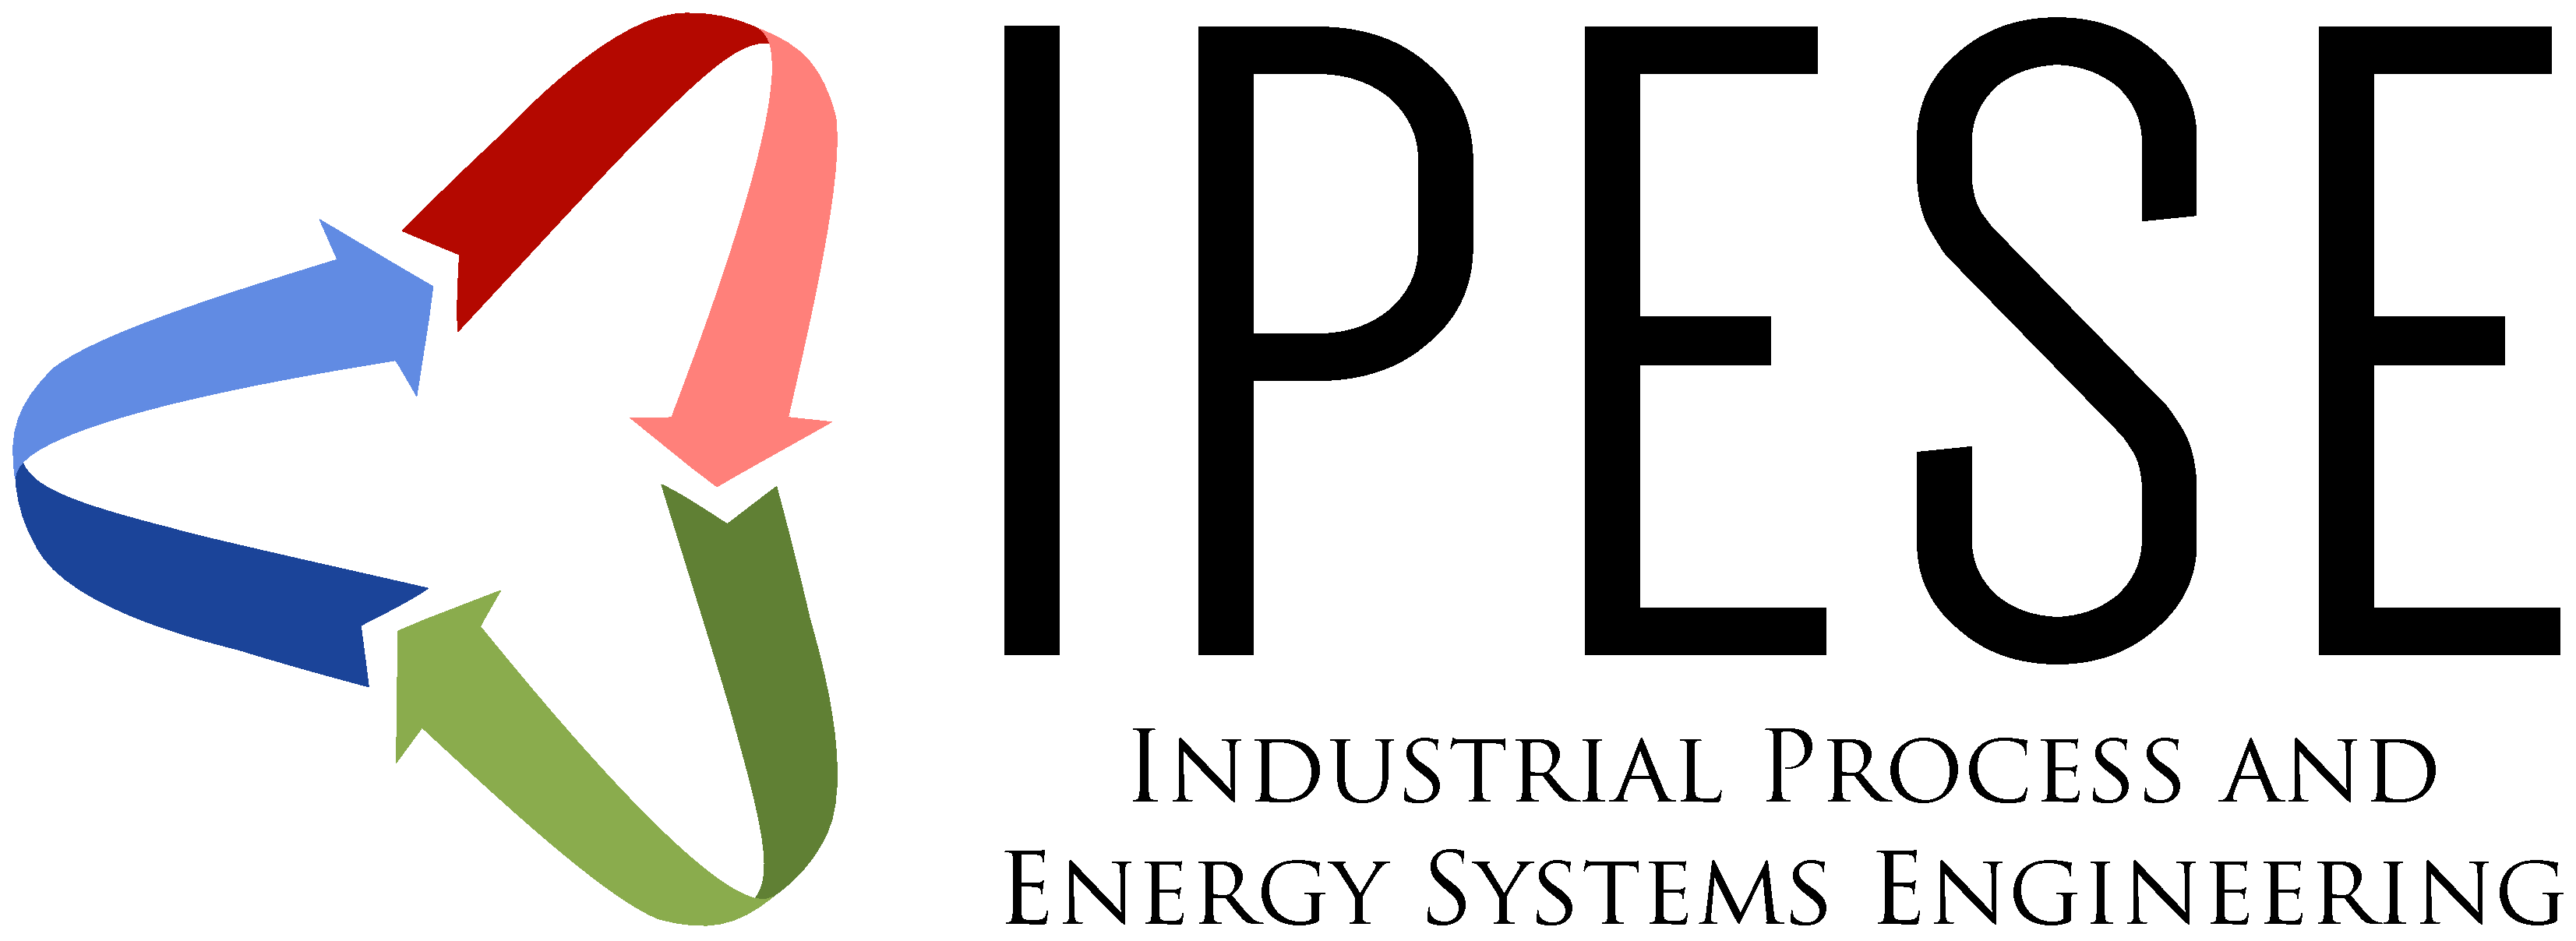
\includegraphics[width=4.6cm]{Logos/logo_ipese.eps}}
\end{figure*}

% To add footnote to the title page
\fancypagestyle{postprintnote}{\fancyhf{}\renewcommand{\headrulewidth}{0pt}\fancyfoot[R]{%
%footer text goes here
}}
\thispagestyle{postprintnote}

\end{titlepage}


% \begin{titlepage}

% \newcommand{\HRule}{\rule{\linewidth}{0.5mm}} % Defines a new command for the horizontal lines, change thickness here

% \center % Center everything on the page
% %----------------------------------------------------------------------------------------
% %	TITLE SECTION
% %----------------------------------------------------------------------------------------

% \HRule \\[0.4cm]
% { \huge \bfseries CO2 Networks}\\[0.4cm] % Title of your document
% { \Large \bfseries --- A Case Study ---}\\[0.4cm] % Title of your document
% \HRule \\[1.5cm]
 
% %----------------------------------------------------------------------------------------
% %	AUTHOR SECTION
% %----------------------------------------------------------------------------------------

% \begin{minipage}{0.4\textwidth}
% \begin{flushleft} \large
% \emph{Authors:}\\
% Tobia \textsc{Wyss} 
% \author[2]{Tobia Wyss\thanks{tobia.wyss@epfl.ch}}
% \end{flushleft}
% \end{minipage}

% ~
% \begin{minipage}{0.4\textwidth}
% \begin{flushright} \large
% \emph{Supervisors:} \\
% Pr. François \textsc{MARECHAL}\\
% \author[1]{Fran\c{c}ois Mar\'echal\thanks{francois.marechal@epfl.ch}}
% Luc  \textsc{GIRARDIN}\\
% Luise \textsc{MIDDELHAUVE}

% \end{flushright}
% \end{minipage}\\[2cm]

% %To add the affiliations
% \affil[1]{Industrial Process and Energy Systems Engineering (IPESE), \'Ecole Polytechnique F\'ed\'erale de Lausanne}
% \affil[2]{Master student, \'Ecole Polytechnique F\'ed\'erale de Lausanne}

% %----------------------------------------------------------------------------------------
% %	LOGO SECTION
% %----------------------------------------------------------------------------------------

% % To add the logos
% \begin{figure*}[!htb]
% \centering
% \subfigure{
\includegraphics[width=4cm]{Logos/logo_epfl.eps}}\hfill
% \quad
% \subfigure{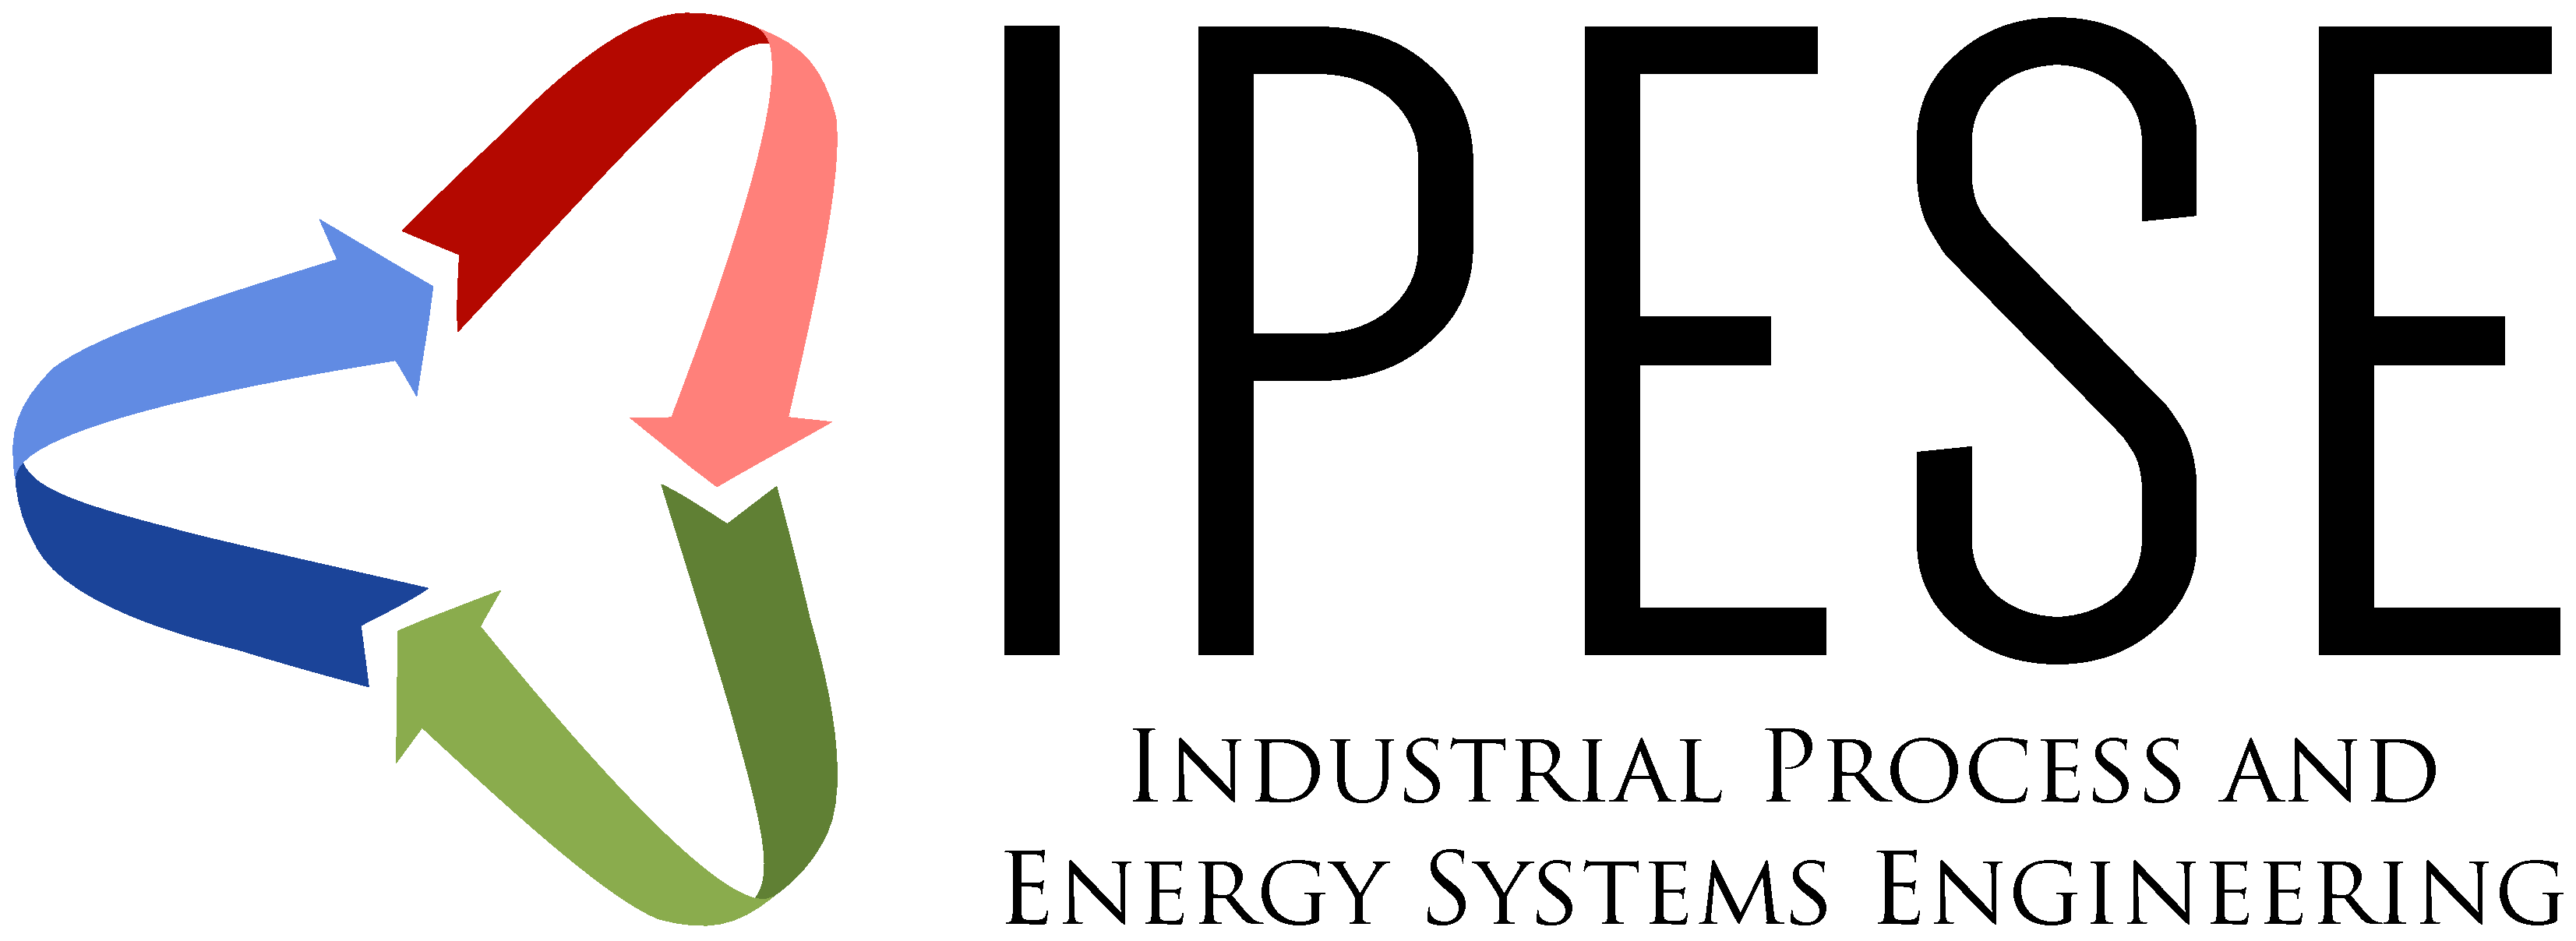
\includegraphics[width=4.6cm]{Logos/logo_ipese.eps}}
% \end{figure*}

% {\let\newpage\relax\maketitle}
% % To add footnote to the title page
% \fancypagestyle{postprintnote}{\fancyhf{}\renewcommand{\headrulewidth}{0pt}\fancyfoot[R]{%
% %footer text goes here
% }}
% \thispagestyle{postprintnote}

% \thispagestyle{empty}
% \clearpage

% \end{titlepage}


%%%%%%%%% Empty page %%%%%%%%%
\newpage
\null
\thispagestyle{empty} % to have a page without page number
\clearpage

%%%%%%%%% TODOS %%%%%%%%%
\listoftodos
\newpage

%%%%%%%%% Contents %%%%%%%%%
\begin{abstract}
District energy systems present a high potential to reduce CO2 emissions caused by cities, thanks to the implementation of large polygeneration energy conversion technologies connected to buildings over a network.
A specific technology, developed by EPFL, using a CO2 network...
A comparative analysis shows that...
\end{abstract}

%%%%%%%%% Contents %%%%%%%%%
\newpage
\tableofcontents
\thispagestyle{empty} 

%%%%%%%%% List of Figures %%%%%%%%%
%\newpage
%\listoffigures
%\thispagestyle{empty}

%%%%%%%%% List of Tables %%%%%%%%%
%\newpage
%\listoftables
%\thispagestyle{empty}


%%%%%%%%% Reset page counter %%%%%%%%%
\setcounter{page}{1}
\renewcommand{\thepage}{\arabic{page}}
\newpage

%%%%%%%%%%%%%%%%%%%%%%%%%%%% CONTENT %%%%%%%%%%%%%%%%%%%%%%%%%%%%%%%%%%%


\section{Introduction}

\subsection{Context}
Today climate change a fact, emissions explosed. We have to reduce...
With the Kyoto protocol, the first international treaty about the fight against climate change, many countries have agreed to drastically reduce CO2 emissions in the coming decades.\\
One crucial sector is the production of heat, which represents a large share of the total greenhouse emissions. This is especially true countries at higher latitudes, i.e. with cold climates. For example in Switzerland the energy demand for space heating and hot water demand of buildings, accounts for around 41\% (96.5 TWh) of the total energy demand of the country, and is still strongly dependent from fossil fuels. If we also include process heat, this figure rises to 54\% (123.9 TWh)\cite{bacherEnergieRespektSchlusselFur2014}. \\
On the other side, the energy demand related to cooling is experiencing an exponential growth. This is, on the one hand, because it is becoming affordable for more people, as income levels rise. On the other hand, this increase is due to global warming. 
There are today 1.6 billion air conditioners (AC) in use, and about 50\% of them are distributed in only two countries: China and USA. In some countries, especially in the Middle East, as well as in parts of the USA, during extremely hot days cooling can represent more than 70\% of peak residential electricity demand. A huge problem with respect to this, is the quality of ACs. The majority of ACs that are sold in large markets, have an efficiency, which is only 50\% or lower than the one of the best products available. This engenders, obviously, an important augmentation of the energy demand. Figure \ref{fig:cooling_energy} shows how the energy demand has tripled since 1990, while the share of cooling energy in total energy use in buildings has risen from 2\% to more almost 7\% \cite{birolFutureCooling2018}. \\ 

\begin{figure}[h!]
	\centering
	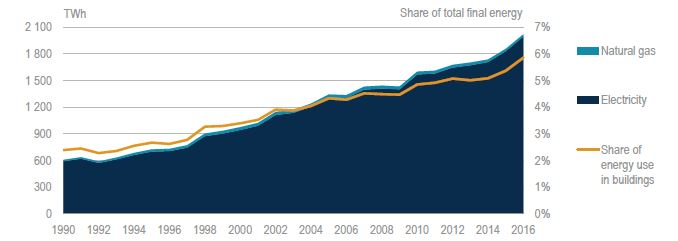
\includegraphics[width=0.7\textwidth]{cooling_energy.JPG}
	\caption{World energy consumption for space cooling in buildings. Source:\cite{birolFutureCooling2018}}
	\label{fig:cooling_energy}
\end{figure}

A study shows that also in Switzerland cooling demand will strongly increase in the next decades, due to climate change. Figure \ref{fig:climat_CH} shows how this is particularly true for modern houses, which are very well isolated and efficient for the winter use. In this case the cooling demand will represent more or less a third of the heating demand\cite{hsluClimaBauPlanenAngesichts2017}.\\

\begin{figure}[h!]
	\centering
	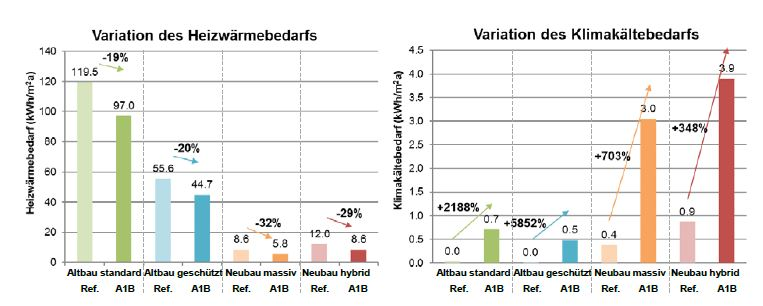
\includegraphics[width=0.7\textwidth]{climat_CH.JPG}
	\caption{The evolution of median values of heating (left) and cooling (right) demand of the fours case studies ("Old building", "Old builing protected", "Solid construction", "Hybrid construction") between the reference period "1995" (1980-2009) and the period "2060" (2045-2074) in Basel. The percentage variations can be attributed to climate change. A1B corresponds to a median scenario developed by the IPCC. Source: \cite{hsluClimaBauPlanenAngesichts2017}}
	\label{fig:climat_CH}
\end{figure}

% Cities have a central role to play in the transition to sustainable energy, as in an urbanized society, they are responsible for more than 70 percent of global energy demand. 

According to the Population Division of the United Nations, the share of the world population living in cities has steadily increased from 34\% in 1960 to 55\% in 2017. Moreover, they prospect that, by 2050, this number will rise to 66\%. In Switzerland, as well as in its neighbouring countries, the percentage of urban population is considerably higher, with 74\% (2017) \cite{unitednationspopulationdivisionWorldUrbanizationProspects}.
The fact that people live more and more in concentrated areas, also mean that the density of energy consumption is rising. This becomes particularly interesting for urban heating and cooling demand, since the high density of heat consumers sets the conditions for efficient  systems, based on district energy networks.\\
The UNEP (United Nations Environment Programme) has identified a big potential in modern district energy systems, as the most effective approach to improve energy efficiency for heating and cooling, and enable the integration of renewable energies. \\
However, these technologies require a high level of technology coordination and planning, since they create more efficient systems that are also more complex to deploy and operate. This is why, further research and technology development are needed in order to foster the spreading of these technologies.

% \textit{Generally, these networks rely on centralized energy conversion technologies supplying heating and/or cooling to the users through a water network. In most of the cases, the supply temperature of these networks is selected, at best, according to the most demanding consumer connected. Thus all the other users are supplied at a temperature beyond their needs - often far beyond their needs. Furthermore, when heating and cooling have to be  supplied, two independent water loops are used. Finally, most of the time, heat discharged by the cooling users in the district cooling network is not transferred to the district heating network, and thus not recovered.} \cite{henchozPotentialRefrigerantBased}

% \textit{On the user side,
% the heat demand of a modern home has reduced significantly,
% so that one can wonder if it is still useful to place
% individual, gas-fired heating units in each home. On the
% supply side, thermal grids offer the opportunity to make
% use of renewable energy or waste heat. Such systems
% can work with far lower temperatures than traditional
% district heating networks. The next step is to make the
% thermal grids interactive, so that users can extract both
% heat and cold from them.}

\subsection{Scope}
The scope of this project is to pursue the study of the application of the CO2 based district energy network technology, proposed by Weber and Favrat\cite{weberConventionalAdvancedCO22010a}. In collaboration with Romande Energie, the utility company of canton Vaud, a feasibility study has to be performed on a specific case study: the residential district Eglantine in Morges. The work will try to answer the main research questions:\\
%developed at the Industrial Process and Energy Systems Engineering (IPESE) group at the École Polytechnique Fédérale de Lausanne (EPFL)
\textit{How does the CO2 district energy network perform - ecologically as well as financially - in the Eglantine district, and under which conditions does it perform better than concurrent solutions?}\\

\textit{What are the characteristics of a typical district that favour the choice of the CO2 district energy network technology?}


\section{Literature review/State of the art}

\subsection{District heating}
The evolution of the technology of district heating (DH) is shown in Figure \ref{fig:4GDH}.
The first District Heatings (DH) have been installed in the 1880s in the USA, using concrete ducts to distribute steam at high temperature, which was then condensated by the consumers. This system was obviously not very efficient, due to the elevated heat losses during transportation, as well as the exergy losses due to the high temperature level. In the early 1930 a second generation was developed, which based on the use of pressurized water, distributed above 100\si{\celsius}. These networks were installed with the purpose of reducing fuel consumption, as well as to integrate the energy generation through CHPs (Combined Heat and Power). The third generation was introduced in the 1980s and it's main difference was the use of a lower distribution temperature (below 100 \si{\celsius}). In those years the main reasons for the installation of DH was security of supply, since they allowed to replace oil with more local and cheaper fuels such as coal, biomass and waste. Moreover, it allowed to use industrial waste heat, as an energy source. Nevertheless, a distribution temperature between 70-100 \si{\celsius} still origins very high heat losses, and it does not allow to integrate a larger number of heat sources. Moreover, also in space heating systems in buildings, there has been an evolution towards lower operating temperatures, reducing the average demand temperature.\\
These were the drivers for the development of the 4th generation, for which networks operate at a temperature between 30-70 \si{\celsius}. This enables a much better integration of the heating system into the global energy system, as it makes it possible to include low temperature sources (geothermal, solar thermal, refrigeration systems or waste heat from data centers).
 
\begin{figure}[h!]
\centering
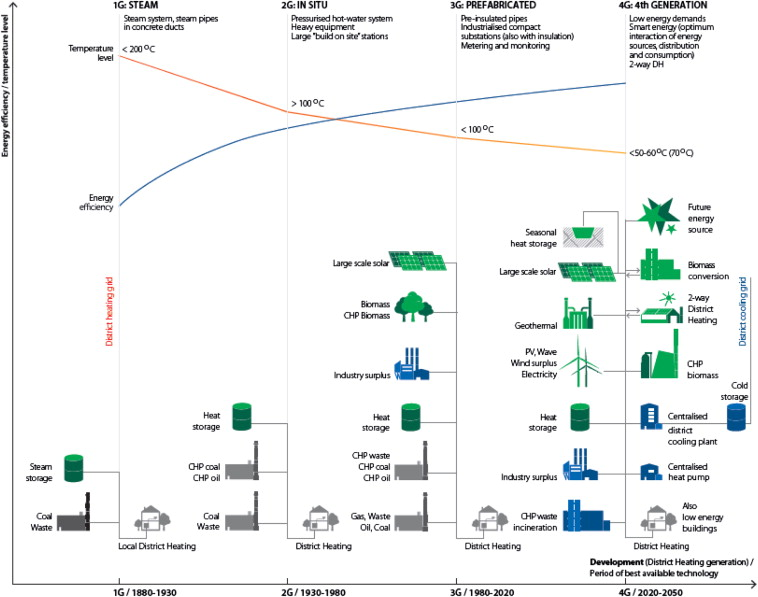
\includegraphics[width=1\textwidth]{4GDH.jpg}
\caption{The evolution of the district heating technology, from the 1st to the 4th generation. Source: \cite{lund4thGenerationDistrict2014}}
\label{fig:4GDH}
\end{figure}

District cooling (DC) networks had a similar development as DH networks, although to a smaller extent. 
% As seen in previous chapter, cooling demand will increase, especially for commercial applications. As for district heating in cold climates, in order to satisfy the future demand, several countries plan to develop the infrastructure for district cooling. For example the city of Dubai, for which air conditioning represents over 70 per cent of electricity consumption, aims to meet 40 per cent of its cooling needs through district
% cooling by 2030, using 50 per cent less electricity than standard air conditioning.\cite{unitednationsenvironmentprogrammeunepDistrictEnergyCities2015}

\subsection{Fifth generation district energy networks}\label{ss:5gden}
The 4th generation of DH technology, has already achieved remarkable success and has been widely applied, especially in Europe. However, the exergy losses of the system are still very high, due to the diversity of heat levels present in the system, limiting its efficiency. Moreover, the integration of DC, which, as it was mentioned beforehand is already important in cities and will become more and more important throughout the next years, needs the installation of a second and separate networks, which leads to high upfront costs. \\
This has lead to the birth of a new technology that uses an even lower distribution temperature (10-25 \si{\celsius}) to provide heating and cooling. In fact, the transfer fluid acts as cold network for cooling purposes and supplies, at the same time, evaporator heat to decentralized heat pumps. This is what is known as the 5th generation DH networks, also known as District Energy Networks (DEN) or District Heating and Cooling (DHC).\\

\todo{write out that part}
The benefits of Fifth Generation District Heating and Cooling include:
\begin{itemize}
	\item flexibility to scale up
	\item zero carbon emission and pollution on site
	\item ability to recycle waste heat
	\item lower insulation needed 
	\item lower depth
	\item economics
	\item lower capital cost of construction
	\item lower running costs
	\item lower maintenance costs
\end{itemize}

This technology has appeared in Switzerland in 2007, and it's mostly known as \textit{anergy network}, or in german \textit{Anergienetz}. To the authors knowledge, there are seven such systems operating by the end of the year 2018\cite{energieschweizFallbeispieleThermischeNetze2018}. A summary of a selection of four of them is shown in Table \ref{tab:anergieCH_sum}, while more detailed information can be found in the Appendix \ref{as:anergy_suisse}.

\begin{table}[h]
\centering
\caption{District energy systems in Switzerland}\vspace{2mm} 
\label{tab:anergieCH_sum} 
\begin{tabular}{llllllll}
\toprule
                                                                                      & \textbf{\begin{tabular}[c]{@{}l@{}}
                                                                                      	Anergienetz \\
                                                                                      	    ETH     \\
                                                                                      	Hönggerberg
                                                                                      \end{tabular}} & \textbf{\begin{tabular}[c]{@{}l@{}}Suurstoffi-\\ Areal\end{tabular}}                             & \textbf{\begin{tabular}[c]{@{}l@{}}Anergienetz \\ Friesenberg (FGZ)\end{tabular}} & \textbf{\begin{tabular}[c]{@{}l@{}}Genève-Lac-\\ Nations (GLN)\end{tabular}} \\
\midrule
\textbf{Location}                                                                     & Zürich                                                                             & Rotkreuz                                                                                         & Zürich                                                                            & Genève                                                                       \\
\textbf{Year of construction}                                                         & 2012 - 2026                                                                        & 2010 - 2020                                                                                      & 2011-2050                                                                         & 2008 - 2016                                                                  \\
\textbf{ERA [m2]}                                                                     & 475'000                                                                            & 172'421                                                                                          & 185'000                                                                           & 840'000                                                                      \\
\textbf{\begin{tabular}[c]{@{}l@{}}Inst. Heating\\ capacity [kW]\end{tabular}}        & 8'000                                                                              & 6'732                                                                                            & 3'930                                                                             & 4'300                                                                        \\
\textbf{\begin{tabular}[c]{@{}l@{}}Heating demand \\ '[MWh/a]'\end{tabular}}          & 28'450                                                                             & 10'619                                                                                           & 35'000                                                                            & 5’000                                                                        \\
\textbf{\begin{tabular}[c]{@{}l@{}}Inst. Cooling\\ capacity [kW]\end{tabular}}        & 6'000                                                                              & 2'327                                                                                            & 3'500                                                                             & 16'200                                                                       \\
\textbf{\begin{tabular}[c]{@{}l@{}}Cooling demand \\ '[MWh/a]'\end{tabular}}          & 26'200                                                                             & 2'364                                                                                            & 80'000                                                                            & 20'000                                                                       \\
\textbf{Distribution fluid}        & water                                                                              & water                                                                                            & water                                                                            & water                                                                       \\
\textbf{Heat source}                                                                  & \begin{tabular}[c]{@{}l@{}}Laboratories\\ waste heat \\ +HP\end{tabular}           & \begin{tabular}[c]{@{}l@{}}Waste heat \\ buildings \\ + PVT (solar th.) \\ +HP\end{tabular}      & \begin{tabular}[c]{@{}l@{}}Waste heat\\ data center+HP\end{tabular}               & Lake water +HP                                                               \\
\textbf{Heat storage}                                                                 & \begin{tabular}[c]{@{}l@{}}Geothermal well \\ field\\ (431 at 200m)\end{tabular}   & \begin{tabular}[c]{@{}l@{}}Geothermal well\\ field \\ (215 at 150 m,\\ 180 at 280m)\end{tabular} & \begin{tabular}[c]{@{}l@{}}Geothermal well\\ field\\ (332 at 250m)\end{tabular}   & None                                                                         \\
\textbf{T of heating pipe}                                                                & 24 \si{\celsius} - 8 \si{\celsius}                                                                       & 25 \si{\celsius} - 8 \si{\celsius}                                                                                     & 28 \si{\celsius} - 8 \si{\celsius}                                                                      & 17 \si{\celsius} - 5 \si{\celsius}                                                                 \\
\textbf{T of cooling pipe}                                                                & 4 \si{\celsius} - 20 \si{\celsius}                                                                       & 4 \si{\celsius} - 17 \si{\celsius}                                                                                     & 4 \si{\celsius} -24 \si{\celsius}                                                                       & 5 \si{\celsius} - 12 \si{\celsius}                                                                 \\
\textbf{\begin{tabular}[c]{@{}l@{}}Tot. investments\\ '[Mio.CHF]'\end{tabular}}       & 37                                                                                 & n/a                                                                                              & 42.5                                                                              & 33                                                                           \\
\textbf{\begin{tabular}[c]{@{}l@{}}
	Tot. COP of heating \\
	  (incl. Pumps…)
\end{tabular}} & 5.8                                                                                & 2.7                                                                                              & 4.1                                                                               & 6.5                                                                            \\
\bottomrule
\end{tabular}
\end{table}


All the anergy networks presented in Table \ref{tab:anergieCH_sum} still base on water as a working fluid. Therefore, they work on sensible heat, which means that a heat exchange is bound to a variation in the fluids temperature. The challenge of these systems is given by the flow rate that is necessary to limit the temperature difference between the inlet and the return temperature of the network.\\
Thus, it could be very interesting to use refrigerants, instead of water, that enable to work with latent heat instead, which means collecting and distributing heat through the condensation, or the evaporation, of the refrigerant. This poses some additional technological challenges, but has also very clear advantages, as it will be shown in the next chapters.\\

%Generally, however, refrigerant based DEN are still at a prototype stage.

\begin{figure}[h!]
\centering
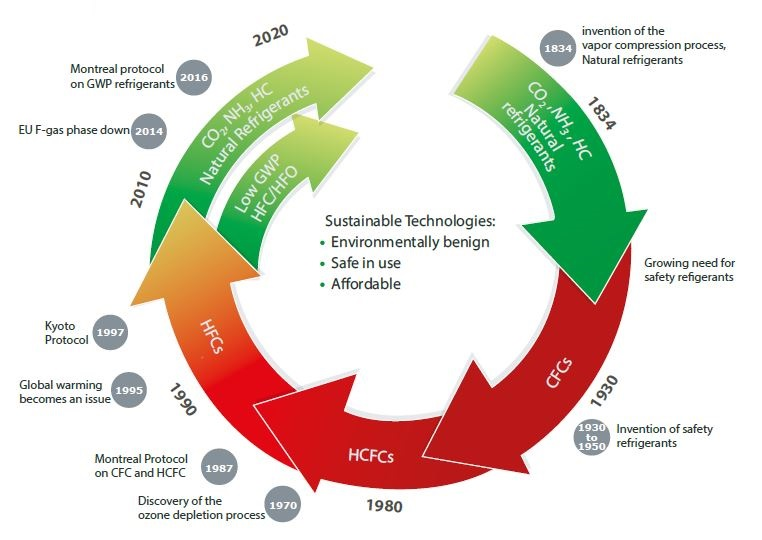
\includegraphics[width=0.75\textwidth]{refrigerants.JPG}
\caption{The historical cycle of refrigerants Source: \cite{danfossRefrigerantOptionsNow2017}}
\label{fig:refrigerants}
\end{figure}

The choice of the refrigerant strongly depends on the application. In function of the operating conditions, three main criteria are evaluated: affordability, safety and environmental impact.
A summary of the history of refrigerants is shown in Figure \ref{fig:refrigerants}.
The Montreal protocol, signed in 1987, designed the phase out of HCFC and CFCs, in order to prevent ozone layer depletion. This boosted the use of HFCs, as a replacement. However, not far later, people realized that despite being less damaging to the ozone layer, they were powerful greenhouse gases. Since 2013, a federal ordinance also strongly restricts the use of these last ones in Switzerland\cite{hydrocarbons21.comSwitzerlandIntroduceHFC}. Also Europe has planned the phase-out of HFC in 2014\cite{europeancommissionforclimateactionEULegislationControl2016}. This means that today the choice of refrigerants is essentially limited to natural refrigerants - as for example CO2 (R744), ammonia (R717) or propane (R290) - and the new environmentally friendly HFOs - as for example the fluorinated propane isomer R1234yf.\\
According to Danfoss\cite{danfossRefrigerantOptionsNow2017}, CO2 will dominate industrial refrigeration, together with ammonia. Already today, this technology is widely used. For instance Migros, Switzerland's largest retail company, opened its first supermarket to use CO2, in a low-temperature subcritical system, in 2002. By today, 411 of the 700 supermarkets in Migros’s portfolio are equipped with transcritical CO2 systems\cite{williamsMigrosDNA2018}.
The choice of CO2 as a refrigerant relies, besides its thermodynamic properties, on the following arguments\cite{cavalliniPROPERTIESCO2REFRIGERANT}:
\begin{itemize}
	\item it is very abundant in the environment and is also waste of a multitude of industrial processes, resulting in very low cost
	\item it is harmless to the biosphere
	\item it is non-flammable and non-toxic
	\item it is an inert gas
\end{itemize}

\subsection{CO2 DEN}

\subsubsection{The technology}
Weber and Favrat \cite{weberConventionalAdvancedCO22010a} proposed a new DEN based on the use of subcritical CO2. 
Also compared with water and HFO R1234yf and proved it best\cite{henchozPotentialRefrigerantBased}.
\todo{rewrite this beginning}
As explained above, a refrigerant based DEN technology allows to store and transfer heat through the latent heat of vaporization of the refrigerant. The operating pressure is chosen in order to obtain the desired temperature in the system. That temperature is selected to be as high as possible to represent a good heat source for the decentralized heating heat pumps - resulting in good COP values -, while still allowing free cooling - avoiding the installation of compression chillers, and thus drastically reduce electricity consumption for space cooling. \\
The network consists of one saturated liquid pipe and of one saturated vapor pipe, both in a saturated temperature range from 12 to 18 \si{\celsius}\cite{suciuEnergyIntegrationCO22018}.
The working principle is shown in Figure \ref{fig:CO2schema}. Heating users can extract heat from the network through condensation of the refrigerant, taken from the vapour pipe. Respectively, cooling users take refrigerant from the liquid pipe and evacuate heat by evaporating it. The heat exchanges between the network and the users occur through condenser-evaporators heat exchangers, which keep the different refrigerant loops isolated\cite{henchozPotentialRefrigerantBased}. The synergy between simultaneous heating and cooling users allows the recovery of waste heat. Most of the time, the required heating and cooling capacity will not be equal, which means that there is the need for a centralized balancing power. Indeed, a central plant is responsible to balance the overall network, by exchanging heat with the environment. For instance, a sole/water or a water/water heat pump can be used for this purpose.\\

%A comparison of the energy performance of two refrigerant based networks, CO2 and HFO R1234yf, and one cold water
%(anergy) network can be found in Ref.:
%S. Henchoz, P. Chatelan, F. Maréchal, and D. Favrat, “Key energy and technological
%aspects of three innovative concepts of district energy networks,” in Proceedings Of
%the 28th International Conference On Efficiency, Cost, Optimization

\begin{figure}[h!]
\centering
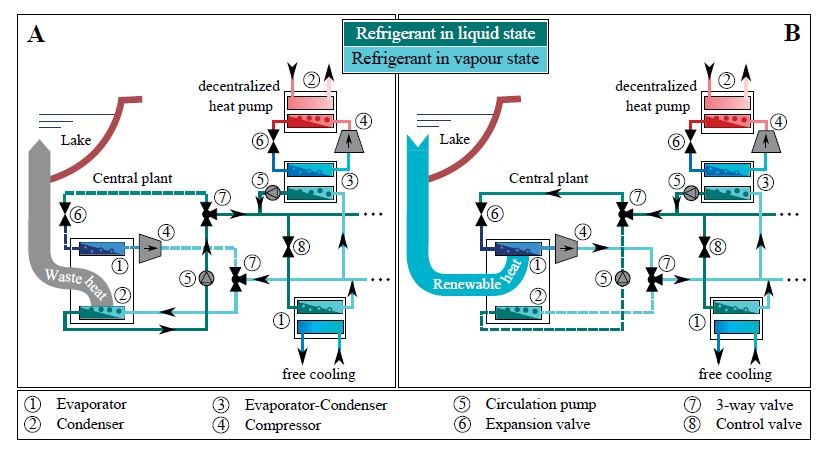
\includegraphics[width=1\textwidth]{CO2schema.JPG}
\caption{Schematics of a refrigerant based district energy network. Part A represents its net cooling operation, and part B its net heating operation. Source: \cite{henchozPotentialRefrigerantBased}}
\label{fig:CO2schema}
\end{figure}

One of the big advantages of this technology, with respect to water based DEN, is the pipes sizing. In fact, given the fact that it works on pressure maintenance instead of a fluid flow, no return pipe is necessary, which results in a slightly shorter total length of installed pipes. Moreover, due to the higher energy density of latent heat, the pipes diameter is drastically reduced. Henchoz et al. compared three different working fluid on the same study case, showing that, while CO2 needs pipes of only 280/330mm (liquid/vapor), R123yf would need 270/700mm and water 625/625mm. Given the low operating temperatures, there are much lower requirements for pipes insulation. While water pipes need to be buried deep enough to prevent damage due to water freezing, in case part of the network had to be stopped during winter, CO2 does not freeze and thus does not require a minimum freeze-safe depth. Henchoz et al. have even imagined installing the pipes inside a sidewalk module, which would drastically simplify maintenance and inspection. \cite{henchozPotentialRefrigerantBased} \\
All the above mentioned advantages of using CO2, result in lower upfront costs, as well as lower maintenance costs.

\textit{\begin{itemize}
	\item flexibility to scale up
	\item zero carbon emission and pollution on site
	\item no chimneys or cooling towers in the city
\end{itemize}}

The main drawback of this technology is the high operating pressure, which situates at about 50 bars, and the safety concerns that could derive from the large amount of CO2 that could escape in case of a major leakage. Nevertheless, as described in \ref{ss:5gden}, CO2 refrigeration networks are already widely used in supermakets, and the technology is considered as safe. \\
\todo{need more drawbacks? or write more about it?}
\textit{Safety issues analyzed \cite{girardinSafetyIssuesCO2based2016}.\\}
\textit{A cold water network is the second best option, although more expensive initially and thus less profitable, it has several advantages in terms of safety and availability of components.}

\subsubsection{Performance}
Henchoz et al.\cite{henchozPotentialRefrigerantBased} performed an analysis of the potential application of a CO2 based DEN in a district in the city of Geneva. A map of the district, called "Rues basses", is shown in Figure \ref{fig:henchoz_gva}.

\begin{figure}[h!]
\centering
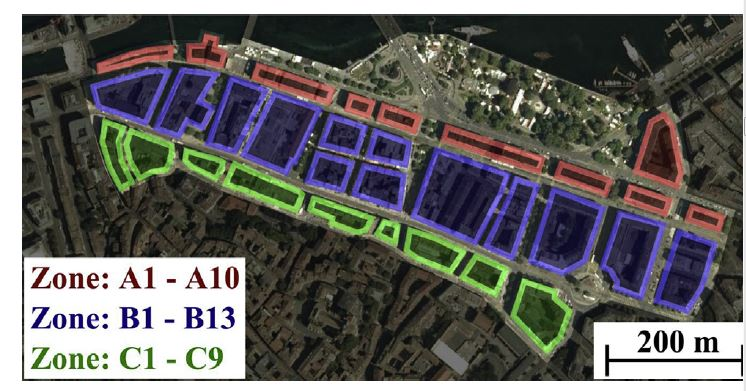
\includegraphics[width=1\textwidth]{henchoz_gva.JPG}
\caption{Representation of the the studied area and of its subdivision into 32 zones. Source: \cite{henchozPotentialRefrigerantBased}}
\label{fig:henchoz_gva}
\end{figure}

Table \ref{tab:henchoz_area} shows the distribution of building affectations - which is important to determine the energy consumption - in the studied area. The total ERA is $687'800 m^{2}$.\\

\begin{table}[h!]
\centering
\caption{Distribution of the energy reference area for the different zones and building affectations}\vspace{2mm}
\label{tab:henchoz_area} 
\begin{tabular}{llll}
	\toprule
	Zones          & Commercial [$m^{2}$ ERA] & Offices  [$m^{2}$ ERA] & Residential  [$m^{2}$ ERA] \\ \midrule
	A1 - A10       & 20'700                   & 89'200                 & 17'700                     \\
	B1 - B13       & 97'000                   & 260'700                & 61'600                     \\
	C1 - C9        & 40'400                   & 62'600                 & 48'100                     \\ \midrule
	Relative share & 23\%                     & 60\%                   & 17\%                       \\ \bottomrule
\end{tabular}
\end{table}

The energy demand of heating and cooling in the studied area is shown in Figure \ref{fig:henchoz_energydemand}. The district presents nearly the same heating demand, as for cooling, but that they happen in different seasons. 

\begin{figure}[h!]
\centering
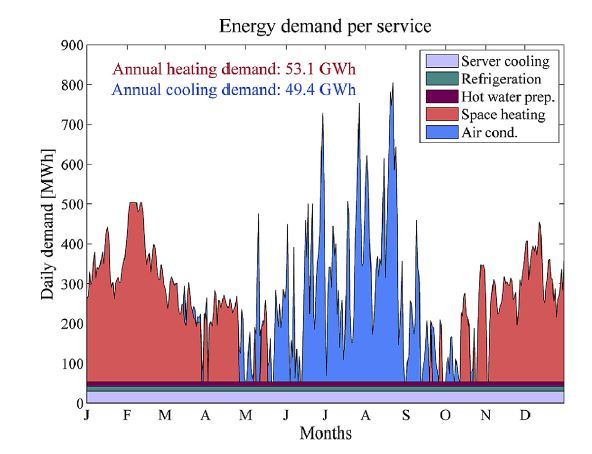
\includegraphics[width=1\textwidth]{henchoz_energydemand.JPG}
\caption{Energy demand for the area studied over the year 2012. Source: \cite{henchozPotentialRefrigerantBased}}
\label{fig:henchoz_energydemand}
\end{figure}

The proposed CO2 based DEN is balanced by a central plant - a heat pump - that exchanges heat with the nearby lake. In order to benchmark the results, this technology has been compared to a traditional heating and cooling system, based on oil boilers and cooled compression chillers.\\
The results are remarkable. In fact, the CO2 based DEN shows a final energy consumption of 10,968 MWh of electricity, which corresponds to a reduction of 84.4 \%, with respect to the reference scenario. 

\begin{figure}[h!]
\centering
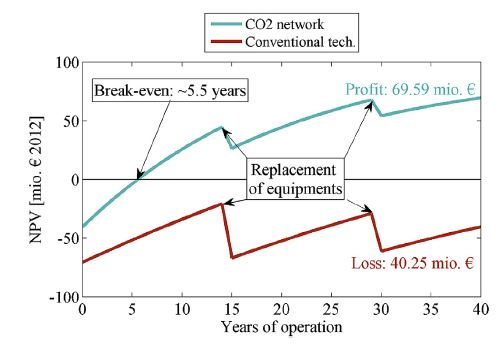
\includegraphics[width=1\textwidth]{henchoz_costs.JPG}
\caption{Evolution of the net present value over the lifetime of the two energy conversion technologies. Source: \cite{henchozPotentialRefrigerantBased}}
\label{fig:henchoz_costs}
\end{figure}

\textit{\begin{itemize}
	\item Such networks can reduce consumption by over 80\%
	\item Exergy efficiencies are typically around 40-45\%
	\item CO2 is the most profitable fluid for district network
	\item A cold water network is the second best option, although more expensive initially
	and thus less profitable, it has several advantages in terms of safety and availability of
	components.
	\item The CO2 variants exhibit a much better compactness than the cold water network.
\end{itemize}
\cite{henchozPotentialRefrigerantBased}}

\subsubsection{Integration in smart energy system}
The integration of high shares of renewable energies represents an important challenge. In fact, it requires a lot of slack to handle the volatile nature of renewable energy sources like wind or sun. On one side, this slack will be mainly given through a smart control of the electricity grid on multiple levels. It starts from the demand side management (DSM) inside households, through optimization at district level, up to a national control. These decentralized grids, or grid controls, are called \textit{smart grids}. With the vast success of heat pumps throughout the last decade, the control of electricity grids is more and more interconnected with the production of heat. This further complexifies the system by adding a level of constraints, but it also opens new levels of control. Indeed, if well designed, a DEN offers an additional level of slack that can be used in combination with the smart grid, multiplying control power.\\
The CO2 DEN offers several possibilities to shift the loads, relieving the grid. 

One one hand, it simplifies the deployment of a smart control of the heat pumps, which can strongly contribute in the DSM. The decentralized heat pumps can make use of a buildings thermal inertia to adapt electricity use to energy availability. CO2 vapor and liquid storage can act as a buffer, enabling load-shifting also for the central plant of the DEN. Sizing of these storage capacities will determine the possible time-span that the shift can achieve. Given the low distribution temperature, this approach also facilitates the storing of heat, as for example in a geothermal field.\\

On the other hand, the use of CO2 as a refrigerant for the network could improve the integration of a power to gas (PtG) system. Indeed, one big challenge in the future, especially in higher latitudes, where seasonal variation are consistent, is to ensure energy supply during winter season, when, due to shorter and weaker solar irradiation, PV panels produce less. It is thus important to find a way to store energy the excess renewable energy during the summer, to the winter.
One solution to do that is PtG, which defines the process of transforming electrical power to a gas, like methane, which is easy to store. To do so, electricity is used to produce hydrogen, which can be combined with CO2 to form Methane, in a process called methanization. Methane can be used during the winter to produce electricity and heat, in a combined heat and power plant (CHP), as for example a SOFC, a gas turbine, or a combination of them. For this reason, PtG is widely studied across Europe and many such plants have already been built.\\ 
Suciu et al. \cite{suciuEnergyIntegrationCO22018} studied the synergy between a CO2 based DEN, decentralized PV and such a PtG system. The CO2 network could be used to store the carbon dioxide, which is captured from CHPs or industrial processes during winter, needed for methanization. At the same time, the DEN can directly use and dispatch the heat produced from the CHPs. In their work, they analyzed the PV area, and thus the investment, required to achieve a completely autonomous energy system, for different European climatic zones. The results showed that in southern Europe the simple available rooftop area is enough to achieve an autonomous system only using solar energy, while in other climatic regions other energy sources are required.

\subsection{Direct-expansion ground source heat pump}\label{ss:dx}
\todo{where to put this section?}

For heat pumps based systems, sourcing heat from the sole, instead of from the ambient air, is a very interesting solution at our latitudes, especially, as it has been seen, for integration of a 5th generation DEN, since it improves heating and cooling COPs, and, to a certain extent, it allows heat storage. In traditional Ground-Source Heat Pumps (GSHP), the heat pump and the ground are connected by means of a closed loop, using water, or a water solution. This system, called the secondary loop GSHP (SL-GSHP), is shown on the right side of Figure \ref{fig:gshp}. However, it has been proved \cite{kruseStatusDevelopmentResearch, guoTechnoeconomicComparisonDirect2012} that the system efficiency can be improved, by allowing to directly expand the refrigerant into the ground and thus let the ground act as a condenser/evaporator. Shown on the left side of Figure \ref{fig:gshp}, this system is called Direct Expansion GSHP (DX-GSHP). 

\begin{figure}[h!]
\centering
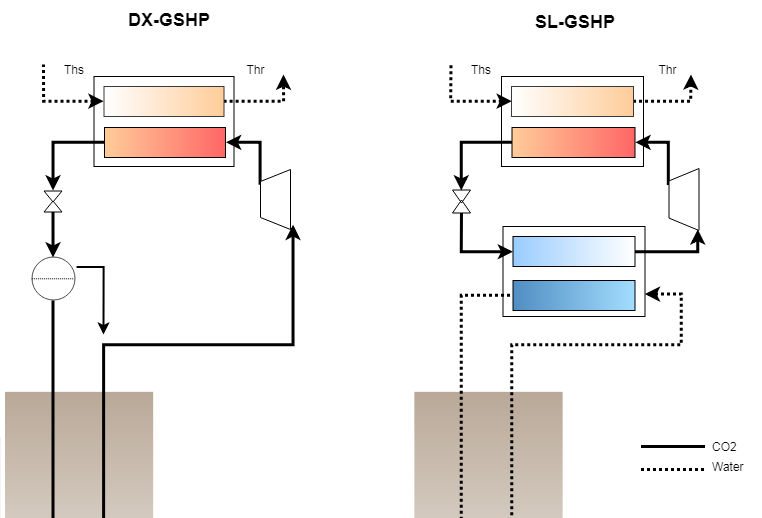
\includegraphics[width=1\textwidth]{GSHP.png}
\caption{A simplified schematics of the two GSHP technologies}
\label{fig:gshp}
\end{figure}

So far, this technology is not so widely spread, mostly because of a more demanding system design and, because of the risk of environmental pollution, when non-natural refrigerants are used. Indeed, literature about DX-GSHP is still scarce, especially for CO2 as a refrigerant. The are only few numerical CO2-DX-GSHP studies \cite{eslami-nejadModelingTwophaseCO2filled2014a,ghazizade-ahsaeeEnergyExergyInvestigation2018,austinParametricStudyPerformance2011,eslami-nejadQuasitransientModelTranscritical2015}, which are not yet sufficient to obtain a scientific appreciation of the technology. Nevertheless several prototypes and experimental set-ups have been built and analyzed \cite{eslami-nejadDetailedTheoreticalCharacterization2018, badacheExperimentalStudyCarbon2018, guoTechnoeconomicComparisonDirect2012}, proving a higher efficiency of the DX, with respect to a SL.\\

On of the main reasons for this efficiency gain is the elimination of the temperature lift of the water loop, which is replaced by a constant temperature phase-change, as well as the elimination of the minimum approach temperature necessary to exchange heat between the SL and the heat pump. This results in a higher COP for the heat pumps. 
Moreover, CO2 presents a higher heat transfer coefficient, which again allows to either reduce the minimum approach temperature, or extract a higher power with respect to an equal exchange surface. The minimum approach temperature has to be determined in function of the thermal permeability of soil and is correlated to the length and total surface of the geothermal probes, as well as the refrigerant flow rate.

\missingfigure{graph Q(T) for DX-GSHP}
 
So the CO2 DEN with DX-GSHP technology is shown in Figure \ref{fig:co2_gshp}

\begin{figure}[h!]
\centering
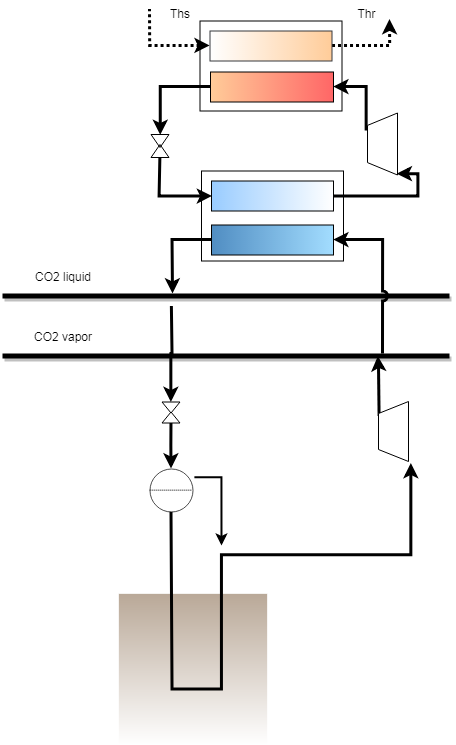
\includegraphics[width=1\textwidth]{CO2-DX-GSHP.png}
\caption{A simplified schematics of the CO2 DEN with DX-GSHP technology}
\label{fig:co2_gshp}
\end{figure}

\todo{DX: choose dTmin for CO2.. arguments against or from articles}

(9) 4/7 for 13 groundT in https://www.sciencedirect.com/science/article/pii/S019689041630975X 
14\si{\celsius}\cite{ghazizade-ahsaeeEnergyExergyInvestigation2018} and \cite{austinParametricStudyPerformance2011}

Assumed temperatures like in ...


\subsection{optimization}

\subsubsection{MILP}
Mixed integer linear programming (MILP) is... 
AMPL a programm, solver using Gurobi, GLPK...
Black box??.....
State variables $X_{state}$
Model $F_{X_{state}}$
Context specification $S_{X_{state}}$
Inequality constraints $G_{X_{state}}$
\todo{find cheatsheet of exam MOES to do that}


%\subsubsection{Genetic algorithms}
%Optimization can be done through empirical algorithms that respect a set of rules. However, it is also possible to explore a space of solutions by reproducing the idea of evolution.
%
%\begin{enumerate}
%\item Create the population
%\item Determine fitness
%\item Select the mating pool
%\item Breed
%\item Mutate
%\item Repeat
%\end{enumerate}
%
%https://blog.sicara.com/getting-started-genetic-algorithms-python-tutorial-81ffa1dd72f9
%https://towardsdatascience.com/evolution-of-a-salesman-a-complete-genetic-algorithm-tutorial-for-python-6fe5d2b3ca35


\subsection{Osmose}
IPESE developed in-house software for this
Lua language
Layers, ETs...
Equations (mass balances, resource balances, heat cascade...)
Creates mod files for ampl optimization
Postcompute to export


Energy conversion technology sizing.
\begin{align}
& f_{u,t} \leq f_{u} \forall \qquad \forall u \in U, \ \forall t \in T  \\
& f_{u}^{min} \cdot y_{u} \leq f_{u} \leq f_{u}^{max} \cdot y_{u} \qquad \forall u \in U\\
\end{align}

For \textit{process units}, only the houses, $y_{u} = f_{u}^{min} = f_{u}^{max} = 1$

Heat cascade
A set of equantions, called heat cascade, makes sure that heat is always transferred from a higher temperature to a lower one, also considering the respective minimum approach temperature for each stream.
\begin{align}
& \sum_{u}^{U} f_{u,t}  \cdot \dot{Q}_{u,t,k} + \dot{R}_{t,k+1} - \dot{R}_{t,k} = 0 \qquad \forall k \in K, \ \forall t \in T \\
& \dot{R}_{t,k} \geq 0 \qquad \forall k \in K, \ \forall t \in T  \\
& \dot{R}_{t,1} = 0 \dot{R}_{t,k+1} = 0 \qquad \forall t \in T  \\
\end{align}
\todo{how is third eq rtk+1 = 0???}

Mass balances
The demand $\dot{m}_{r,u,t}^{+}$ and the supply $\dot{m}_{r,u,t}^{-}$ of resource $r in R$ of each unit $u in U$ is computed.
\begin{align}
& \dot{M}_{r,u,t}^{-} = \dot{m}_{r,u,t}^{-} \cdot f_{u,t} \qquad \forall r \in R, \ \forall u \in U, \ \forall t \in T \\
& \dot{M}_{r,u,t}^{+} = \dot{m}_{r,u,t}^{+} \cdot f_{u,t} \qquad \forall r \in R, \ \forall u \in U, \ \forall t \in T  \\
\end{align}
The balance of each resource has to be respected.
\begin{equation}
\sum_{u}^{U} \dot{M}_{r,u,t}^{-} = \dot{M}_{r,u,t}^{+} \qquad \forall r \in R, \ \forall t \in T
\end{equation}
Electricity is also balanced
\begin{equation}
\dot{El}_{houses}^{+} + \dot{El}_{heating}^{+} + \dot{El}_{cooling}^{+} + \dot{El}_{grid}^{+} = \dot{El}_{PV}^{-} + \dot{El}_{grid}^{-}
\end{equation}

Opitmization function

\begin{align}
& min \left( TotalCost \right)  = min \left(  CAPEX + OPEX \right) \\
& min \sum_{u}^{U} ... \\
\end{align}

\begin{align}
& min \left( Operating cost \right) \\
& min \sum_{u}^{U} \left[ \sum_{t = 1}^{T} \left( c_{u}^{op1} \cdot y_{u,t} + c_{u}^{op2} \cdot f_{u,t} + C_{el}^{-} \cdot \dot{El}_{grid,t}^{-} - C_{el}^{+} \cdot \dot{El}_{grid,t}^{+} \right) \cdot t_{t}^{op} \right] \\
\end{align}

where $c_{u}^{op1}$ and $c_{u}^{op1}$ are the respectively the fixed and the variable operating cost, and $C_{el}^{-}$ and $C_{el}^{+}$ are the buying and selling price of electricity.


\section{Methodology}

\subsection{Investment cost function}
\todo{Take explanation from "MOES EPFL Buildings" report line 127}
\begin{equation}
C_{pex} = \frac{I_{t}}{I_{t,ref}} \cdot 10^ {(k_{1,ex} + k_{2,ex} \cdot \log(A_{ex}))}
\end{equation}

\begin{equation}
CBM_{ex} = C_{pex} \cdot FBM_{ex} \cdot e 
\end{equation}

The annuities are calculated with the annualization factor ($af$) by the following formula, where $n$ is the assumed lifetime of the equipment, and $i$ the interest rate. 

\begin{align}
	& IC_{yearly,ex} = CBM_{ex} \cdot af 
	& af = \frac{i \cdot (1 + i)^n}{(1 + i)^n - 1}
\end{align}

\subsection{Minimum approach temperature}
Bigger area allows a smaller dTmin, which increases the investment costs but lowers the operating costs, due to the higher COP, and the other way around. So an optimum can be found for each specific application.

Then optimization of dTmin in function of total costs minimization, with help of the following equations. Assumed counter-flow heat exchanger 
\begin{equation}\label{eq:HEX_area}
    A_{ex} = \frac{Q_{ex}}{U \cdot LMTD}
\end{equation}
\begin{equation}\label{eq:LMTD}
    LMTD= \frac{(T_{Hot,in } - T_{cold,out }) - (T_{Hot,out } - T_{cold,in }) }{ \log{ (\frac{T_{Hot,in } - T_{cold,out }}{T_{Hot,out } - T_{cold,in }} ) }}
\end{equation}
And the overall heat transfer coefficient is given by \cite{huExtremumSeekingControl2015}
\begin{equation}\label{eq:alpha}
    U= \frac{1}{ \frac{1}{h_{(hot)} } + \frac{\Delta x_{wall}}{k_{wall}} \frac{1}{h_{(cold)}} }
\end{equation}
where $h_{(hot)}$ and $h_{(cold)}$ are the heat transfer coefficient of the hot and cold fluid. Heat resistivity of heat exchanger plates are neglected.

The optimization is done on water refrigerant hp, with values (ic, Q, COP) from space heating. 
CO2 dTmin is calculated maintaining same Area as for ref hp.

for CO2 from this paper\cite{ohFlowBoilingHeat2011}.
Validated also by 
This paper shows R134a and R134yf have same heat transfer coefficient\cite{wangOverviewHeatTransfer2013}, comparison with CO2 done in \cite{mastrulloComparisonR744R134a2009}.
Values are for a diameter and heat flux that could correspond (d = 4.5mm and 20kW/m2)
Also a list of previous studies

\begin{table}[h!]
\centering
\caption{Heat transfer coefficients found in literature}\vspace{2mm}
\label{tab:alphas} 
\begin{tabular}{llll}
	\toprule
	Fluid             & Water & R134yf & R744 \\ \midrule
	$h [W/(mK)]$ & 600   & 3000   & 7000 \\ \bottomrule
\end{tabular}
\end{table}

Thus following $\Delta T_{min}$ are have been calculated and used for heat exchanges in the model.
\begin{table}[h!]
\centering
\caption{Minimum approach temperatures used for heat exchanges in the model}\vspace{2mm}
\label{tab:dtmins} 
\begin{tabular}{lllll}
\toprule
	$\Delta T_{min}$ [K] & Ground & Water & R744 & R1234yf \\
	Water                & 14     & -     & -    & -       \\
	R744                 & 6.8    & 3.46  & 0.8  & -       \\
	R1234yf              & -      & 4     & 1.4  & 2.3    \\ \bottomrule
\end{tabular}
\end{table}


\subsection{Exergy}
The exergy of a heat transfer is defined as the maximum amount of work that can be extracted from it, through reversible transformations that exchange with the environment. Thus the calculation of exergy losses is a very interesting indicator to analyze a given process or system, since it expresses the quality and the efficiency with which the system operates, with respect to the maximum possible. Therefore, these values are always lower than 100 \%. \\

The maximum work that can be extracted is derived from the first two thermodynamic principles, and is given by the following formula:
\begin{equation}
    \dot{E}^{-}_{max} = \sum_{i} \dot{Q_i}^{+} (1 - \frac{T_{a}}{T_i} ) + \sum_{r} \dot{M}_{r}^{+} (h_{r} - T_{a} s_{r})    
\end{equation}

In order to compute the exergy losses the general approach that can be used is the following:
\begin{equation}
    \dot{L} = \dot{E}^{-}_{max} - \sum_{j}\dot{E}^{-}_{j} \geq 0
\end{equation}

In our case
\begin{align}
    & \eta_{exergy} =  \frac{\dot{Q}_{cold,a} + \dot{Q}_{hot,r} + \dot{E}_{grid}^{-}}{\dot{Q}_{cold,r} + \dot{Q}_{hot,a} + \dot{E}_{grid}^{+}}  \\
    & \dot{L} = (1-\eta_{exergy})(\dot{Q}_{cold,r} + \dot{Q}_{hot,a} + \dot{E}_{grid}^{+})
\end{align}

\subsection{Typical days}
\todo{methodology typical days}
The optimization of an energy system is commonly performed over the time span of one year, in order to account for the different seasons. However, this requires a very long computing time, given the high number of timesteps. Thus, it is used to group similar days, according to a set of parameters as for example temperature or irradiation, into so called typical days. The days can be clustered in different ways. It can be chosen to compute an average day for each month or some machine learning clustering algorithm can be used to group the days into the desired number of clusters.
The resulting typical days correspond to a period $p$, with a number of times $t$, as explained in section \todo{missing ss ref}. In order to account for the data compression, a value called $occurrence$ indicates how many times a given typical day occurs, i.e. how many times a given period occurs.

\subsection{Energy technology models}\label{ss:et}

\subsubsection{Heat pumps - basic (Carnot)}\label{sss:hp_carnot}
A simple model can be implemented with the following equations:
Basic Carnot cycle model with efficiency.
\begin{equation}
    \dot{E}_{compressor} = \frac{\dot{Q}_{evap}}{COP_{real}-1} = \frac{\dot{Q}_{evap}}{COP_{theoretical} \cdot \eta_{COP} - 1} = \frac{\dot{Q}_{evap}}{\eta_{COP} \cdot \frac{T_{c} – T_{h}}{T_{c}} -1} 
\end{equation}
where $\eta_{COP}$ is the Carnot efficiency and $\dot{Q}_{evap}$ the heat delivered by the heat pump. \\
\todo{table with eta COP values?}
\todo{how much of this do i have to explain? do i maintain it somewhere in the results to show how much better it is with cycle?}

\subsubsection{Heat pumps - detailed (Thermodyn.)}\label{sss:hp_thermo}
However, given the comparison between new and efficient technologies, the differences of performance are relatively small and it might be necessary to provide a more accurate model of the heat pumps, that are able to correctly represent and calculate the operating cycles and conditions. This can be done like this...
Given cycle:

\begin{figure}[h!]
	\centering
	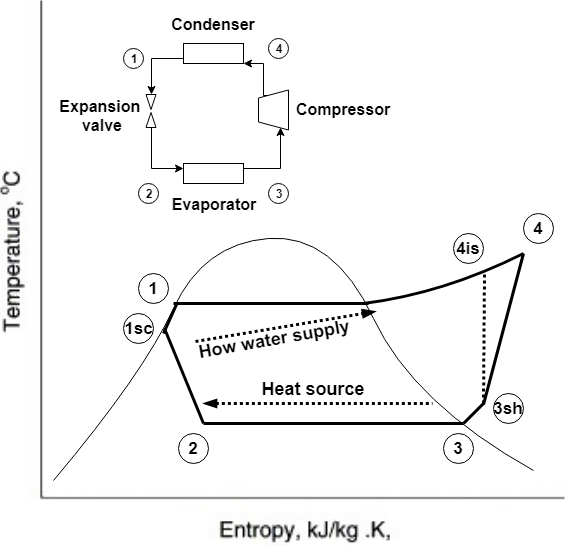
\includegraphics[width=0.6\textwidth]{HP_cylce_ref.png}
	\caption{Temperature–entropy diagram of a R134yf based heat pump system.}
	\label{fig:hp_ref}
\end{figure}

Thermodyn model follows following procedure:
\begin{description}
    \item[1] calculate state in point (x) knowing the evaporation temperature $T_{evap}$, defined in function of heat source temperature $T_{source}$, and assuming saturated liquid
    \item[1sc] subcooled, using same P
    \item[3] calculate state in point (x) knowing the evaporation temperature $T_{cond}$, defined in function of heat demand temperature $T_{heat demand}$, and assuming saturated vapor
    \item[3sh] superheated at evaporator using same P
    \item[2] calculate state at valve outlet, assuming isenthalpic expansion, with $H_{1sc}$ and $P_{3}$
    \item[4is] calculate state for isentropic compression with $P_{1}$ and $S_{3sh}$
    \item[4] calculate state after real compression, given $P_{1sc}$ and $H_{4} = H_{3sh} + \frac{H_{4is} - H_{3sh}}{\eta_{c,is}}$, where $\eta_{c,is}$ is the compressors isentropic efficiency. 
\end{description}

In Osmose, these values are calculated with help of \textit{Coolprop}, which is an open-source database of fluid and humid air properties that allows to calculate operating conditions for a large number of fluids and refrigerants. Thanks to a \textit{lua wrapper}, which is a \textit{lua} module that provides an API to the external software, \textit{Coolprop} is called inside Osmose.

with respectively 1 and 2 \si{\celsius} of superheating and subcooling at the outlet of the heat exchanger \cite{}.
\todo{missing reference for superheat and subcool temp}

The compressor is a crucial component for the design of a heat pump, since it has the largest share of impact on the energy efficiency. To calculate its efficiency, the model of Hu et al.\cite{huExtremumSeekingControl2015} has been used. The shaft power can be computed in function of the isentropic efficiency ($\eta_{is}$) by:
\begin{equation}
W_{shaft} = \frac{\dot{m}(h_{d,is}-h_{s})}{\eta_{is}} 
\end{equation}
where $h_{d,is}$ is the isentropic discharge enthalpy and $h_{d}$ is the suction enthalpy. The compressors input power is expressed in function of its mechanical efficiency ($\eta_{is}$) by:
\begin{equation}
E_{comp} = \frac{W_{shaft}}{\eta_{mech}}  
\end{equation}
The efficiency of the compressor is thus calculated as:
\begin{equation}
\eta_{comp} = \frac{\text{isentropic work of compression}}{\text{actual work of compression}} = \frac{\dot{m}(h_{d,is}-h_{s})}{E_{comp}} = \eta_{is}\eta_{mech} 
\end{equation}

The numerical values of those efficiencies are strongly dependent from the ratio between the pressure of discharge $P_{d}$ and the pressure of suction $P_{s}$ of the compressor.They can be computed with help of the relations obtained by Li et al.\cite{liPerformanceCharacteristicsR1234yf2014}:
\begin{align}
& \eta_{mech} = 0.85\\
& \eta_{is} = 0.874-0.0134\cdot(\frac{P_{d}}{P_{s}})\\
\end{align}
		
The expansion of the refrigerant in the expansion valve is assumed to be isenthalpic. 


\subsubsection{Heat pump CO2}\label{sss:hp_CO2}
In traditional heat pumps, the heat delivery occurs through condensation of the refrigerant, which happens at a fixed temperature. This originates high exergy losses, especially in processes were a high temperature lift is needed in the gas cooler.\\
Some refrigerants have the particular property of having a very low critical point. One very interesting refrigerant, also as explained in Section \ref{label} for environmental reasons, is CO2 - technically know as R744 - which has a critical point at 74 bars and 31 \si{\celsius}\cite{cavalliniPROPERTIESCO2REFRIGERANT}.

The operating cycle can be seen in Figure \ref{fig:hp_CO2}, represented on the temperature-entropy diagram. The different steps of the process are explained hereafter: 
\begin{itemize}
\item 1 - 2 Expansion to low pressure
\item 2 - 3 Evaporation by cooling down the heat source
\item 3 - 3sh Superheating in evaporator
\item 3sh - 4 Compression to transcritical pressure
\item 4 - 1 Gas cooling in transcritical area, to heat water
\end{itemize}

Even though the technological development is slowly closing the gap, CO2 compressors have lower isentropic efficiency and lower volumetric efficiency than subcritical ones\cite{sarkarSimulationTranscriticalCO22006}. This comes from the high irreversibility caused by the superheated vapor horn and the high throttling losses\cite{yangTheoreticalExperimentalInvestigation2016}. 
However, transcritical operation also allows heat to be exchanged on a varying temperature, and the heat pump can be designed to fit the heat demand stream, optimizing exergy efficiency. This is particularly interesting in exchanges that require high temperature lifts, as in the case of domestic hot water heaters. In fact, this can be seen in Figure \ref{fig:hp_CO2}, between point 2 and 3. Note that, as there is no phase change, the heat exchanger is called gas cooler, instead of condenser.\\

\todo{superheating in CO2 hp? how much?}

\begin{figure}[h!]
\centering
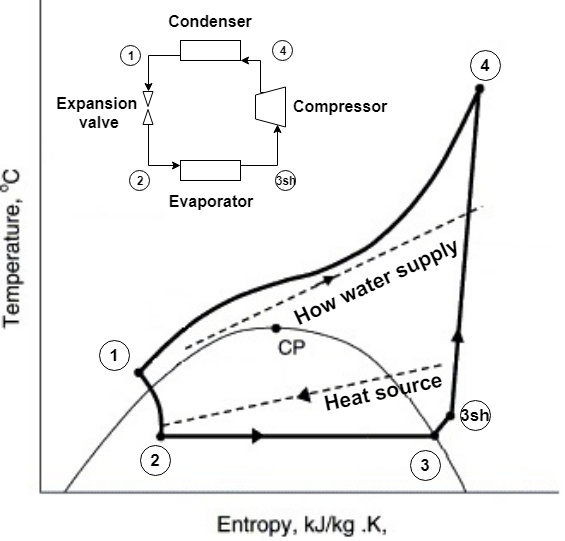
\includegraphics[width=0.6\textwidth]{HP_cylce_CO2.png}
\caption{Temperature–entropy diagram of a trans-critical CO2 heat pump system for a domestic hot water production. Source: \cite{kimPerformanceTranscriticalCO22005}}
\label{fig:hp_CO2}
\end{figure}

For the transcritical CO2 heat pump, the numerical values of the compressor efficiencies computed with help of the relations obtained by Wang et al \cite{wangExperimentalInvestigationAirsource2013}:
\begin{align}
	& \eta_{mech} = 0.64107+0.07487\cdot(\frac{P_{d}}{P_{s}})\\
	& \eta_{is} = 0.8014-0.04842\cdot(\frac{P_{d}}{P_{s}})\\
\end{align}

Stene shows that COP for CO2 hp stays about the same for SH and DHW, because with supercritical condenstion we have a much higher $\eta_{COP}$.\cite{steneINTEGRATEDCO2HEAT2007}


\section{Eglantine}
In the framework of the collaboration between Romande Energie and IPESE, a case study shall bring a concrete numerical case study into the discussion. For this, Romande Energie has chosen a real life example of a district in the city of Morges. This district is in the planning phase, and Romande Energie had worked on it, in order to participate in the call for tender. This case study shall be fertile ground to discuss the CO2 DEN technology and it's role in the future energy systems in Switzerland and, more particularly, in the future plans of Romande Energie.

\subsection{Case-study}
\subsubsection{Context}

\begin{figure}[h!]
\centering
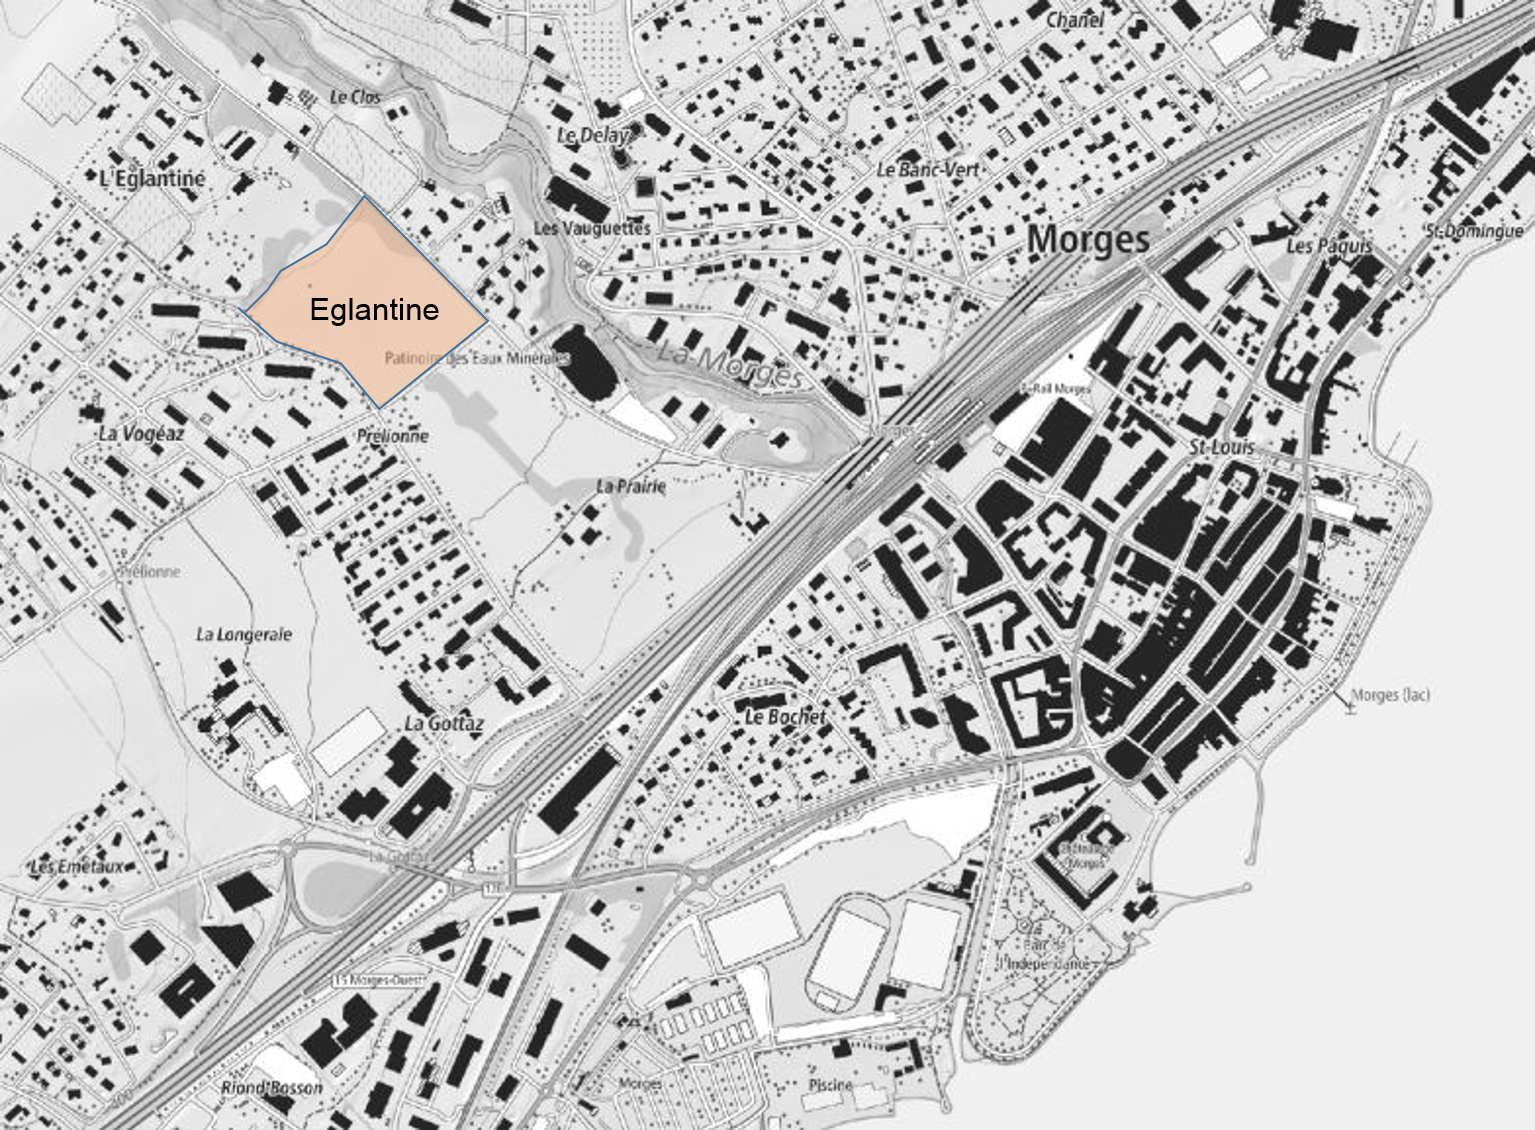
\includegraphics[width=1\textwidth]{morges.png}
\caption{Localization of the terrain, at the town scale. Source: www.geo.vd.ch}
\label{fig:morges}
\end{figure}

The “Eglantine” is a terrain in the western part of the city of Morges, as shown in Figure \ref{fig:morges}. It is located in proximity of the key urban facilities, as well as it is close to the countryside. This terrain, which was partly used for agriculture, and partly covered by rich vegetation, belongs to the municipality, who is planning to use it for the urban expansion. At the municipality, they had the vision of building a new district, which would be planned to be exemplary in the sustainable development. After many years of revising and fine-tuning the land-use plan and its vision for the future, in the beginning of 2016, the commune launched a call for tender for the planning of the different aspects of the district. The call for tender regarding the energy system was opened by Losinger Marazzi the 1st December 2017, with a due date the 31 January 2018. The contract with the winner, unknown to the author, has been signed in the end of March 2018. \\

The call for tender requires the development of a complete energy system, including thermal and electrical energy. Estimated data about the buildings is provided, as seen in Table \ref{tab:ppa_summary}. Those are based on the following assumptions:
\begin{itemize}
    \item All buildings are certificated Minergie 2017
    \item Space heating and hot water energy demand follow the SIA 380/1 and SIA 2031 norms
    \item Air ventilation is defined according to Minergie 2017 principles.
    \item Installed power values are calculated according to SIA 2024 norm
\end{itemize}

\subsubsection{Buildings}
The district, which will host around 1'500 people, is composed of thirteen buildings, as shown in Figure \ref{fig:ppa_buildings}, which account for a total energy reference area (ERA) of around $47'000 m^{2}$. The details are shown in Table \ref{tab:ppa_summary}.\\
The buildings include, beside the residential use, also a small share of commercial and catering use, which are associated with different energy needs. There is also a small swimming pool, located in building one. The use of the buildings is shown in Table \ref{tab:ppa_buildinguse}.
\todo{where does the percentages come from? did not find them in call for tender}

\begin{table}[h!]
\centering
\caption{Estimated energy demand in call for tender}\vspace{2mm}
\label{tab:ppa_summary} 
\begin{tabular}{lrrrrr}
\toprule
\textbf{Building} & \begin{tabular}[c]{@{}l@{}}\textbf{Energy Ref.} \\ \textbf{Area (ERA)}\end{tabular} & \textbf{Inhabitants} & \begin{tabular}[c]{@{}l@{}}\textbf{Space Heating} \\ \textbf{(SH)}\end{tabular}                                             & \begin{tabular}[c]{@{}l@{}}\textbf{Hot Water} \\ \textbf{(DHW)}\end{tabular} & \textbf{TOTAL}     \\
         &                                                                        &             & \begin{tabular}[c]{@{}l@{}}MIINERGIE\\ simple flux\end{tabular} & SIA 380/1       &           \\
         & [m2]                                                                   &             & [kWh/yr]                                                        & [kWh/yr]        & [kWh/yr]  \\
         \midrule
1        & 8'200                                                                  & 273         & 245'180                                                         & 170'833         & 416'013   \\
2        & 2'615                                                                  & 76          & 82'308                                                          & 50'104          & 132'412   \\
3        & 2'415                                                                  & 70          & 76'328                                                          & 45'938          & 122'266   \\
4        & 2'780                                                                  & 92          & 83'122                                                          & 57'917          & 141'039   \\
5        & 3'700                                                                  & 116         & 113'246                                                         & 74'306          & 187'552   \\
6        & 1'500                                                                  & 50          & 44'850                                                          & 31'250          & 76'100    \\
7        & 2'870                                                                  & 83          & 90'652                                                          & 54'653          & 145'305   \\
8        & 2'500                                                                  & 83          & 74'750                                                          & 52'083          & 126'833   \\
9        & 4'225                                                                  & 140         & 126'328                                                         & 88'021          & 214'349   \\
10       & 4'455                                                                  & 148         & 133'205                                                         & 92'813          & 226'018   \\
11       & 4'190                                                                  & 139         & 125'281                                                         & 87'292          & 212'573   \\
12       & 2'300                                                                  & 76          & 68'770                                                          & 47'917          & 116'687   \\
13       & 2'300                                                                  & 76          & 68'770                                                          & 47'917          & 116'687   \\
14       & 2'300                                                                  & 76          & 68'770                                                          & 47'917          & 116'687   \\
\midrule
\textbf{TOT}      & \textbf{46'350}                              & \textbf{1'498}       & \textbf{1'401'559}      & \textbf{948'958}         & \textbf{2'350'521} \\
\bottomrule
\end{tabular}
\end{table}
\begin{table}[h!]
\centering
\caption{Estimated use of buildings in call for tender}\vspace{2mm}
\label{tab:ppa_buildinguse}
\begin{tabular}{lllll}
\toprule
\textbf{Building} & \textbf{Multidwelling} & \textbf{Retail} & \textbf{Restaurant services} & \textbf{Indoor swimming pool} \\
                  & \textbf{[\%]}               & \textbf{[\%]}      & \textbf{[\%]}          & \textbf{[\%]}              \\
                  \midrule
\textbf{1}        & 89.58\%                     & 3.10\%             & 4.42\%                 & 2.89\%                     \\
\textbf{2}        & 97.54\%                     & 2.46\%             & 0.00\%                 & 0.00\%                     \\
\textbf{3}        & 100.00\%                    & 0.00\%             & 0.00\%                 & 0.00\%                     \\
\textbf{4}        & 100.00\%                    & 0.00\%             & 0.00\%                 & 0.00\%                     \\
\textbf{5}        & 93.19\%                     & 6.81\%             & 0.00\%                 & 0.00\%                     \\
\textbf{6}        & 95.79\%                     & 4.21\%             & 0.00\%                 & 0.00\%                     \\
\textbf{7}        & 95.79\%                     & 4.21\%             & 0.00\%                 & 0.00\%                     \\
\textbf{8}        & 100.00\%                    & 0.00\%             & 0.00\%                 & 0.00\%                     \\
\textbf{9}        & 100.00\%                    & 0.00\%             & 0.00\%                 & 0.00\%                     \\
\textbf{10}       & 100.00\%                    & 0.00\%             & 0.00\%                 & 0.00\%                     \\
\textbf{11}       & 100.00\%                    & 0.00\%             & 0.00\%                 & 0.00\%                     \\
\textbf{12}       & 100.00\%                    & 0.00\%             & 0.00\%                 & 0.00\%                     \\
\textbf{13}       & 100.00\%                    & 0.00\%             & 0.00\%                 & 0.00\%                     \\
\textbf{14}       & 100.00\%                    & 0.00\%             & 0.00\%                 & 0.00\%                     \\ \midrule
\textbf{Tot}	  & 97.08 \%					& 1.63 \%			& 0.78 \%					& 0.51 \%					\\
\bottomrule
\end{tabular}
\end{table}

\begin{figure}[h!]
\centering
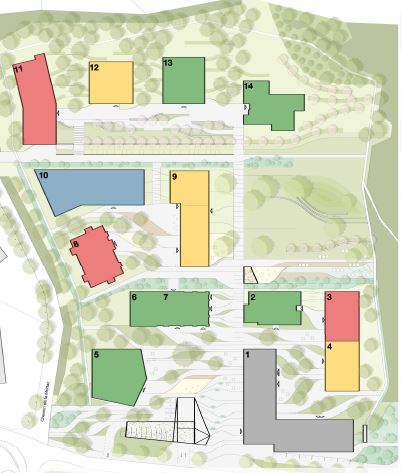
\includegraphics[width=0.45\textwidth]{ppa_buildings.JPG}
\caption{Map of the planned Eglantine district}
\label{fig:ppa_buildings}
\end{figure}

The energy profile of the buildings is calculated according to Minergie standard, as well as the SIA norms. Given the annual energy demand for space heating and hot water, as shown in Table \ref{tab:ppa_summary}, the monthly profile is shown in Figure \ref{fig:ppa_energydemand}.

\begin{figure}[h!]
\centering
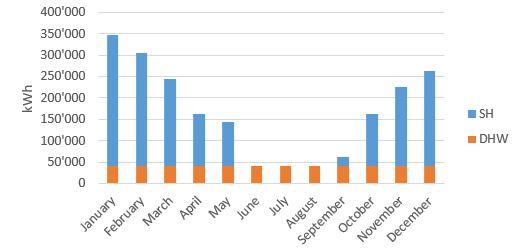
\includegraphics[width=1\textwidth]{ppa_energydemand.JPG}
\caption{Annual energy distribution for space heating and hot water}
\label{fig:ppa_energydemand}
\end{figure}

\todo{cooling demand?}
\todo{typical days graph and results, done as explained in methodology}

\subsubsection{Pre-studies}
Some pre-studies have been commissioned by the land-owner, in order to give, on an indicative basis, the sizing of the energy system. These studies have been realized by external engineering firms and the results are contained in the call for tender. The studied parameters include the sizing for heat pumps, geothermal wells, as well as PV, and are shown in Table \ref{tab:ppa_prestudy}.
\begin{table}[h!]
\centering
\caption{Estimated sizing of energy system in call for tender}\vspace{2mm}
\label{tab:ppa_prestudy} 
\begin{tabular}{lllll}
\toprule
\textbf{Building} & \textbf{PV}    & \textbf{HP}    & \multicolumn{2}{l}{\textbf{Geothermal}} \\
         &       &       & \textbf{Nb. wells}        & \textbf{Depth}        \\
         & \textbf{[kWp]} & \textbf{[kW] } &                 & \textbf{[m] }         \\
         \midrule
1        & 46    & 223   & 13              & 284          \\
2        & 45    & 70    & 4               & 291          \\
3        & 35    & 64    & 4               & 269          \\
4        & 33    & 76    & 5               & 250          \\
5        & 49    & 100   & 6               & 276          \\
6        & 55    & 41    & 3               & 225          \\
7        & 55    & 77    & 5               & 256          \\
8        & 37    & 68    & 4               & 281          \\
9        & 66    & 115   & 7               & 271          \\
10       & 0     & 121   & 7               & 286          \\
11       & 59    & 114   & 7               & 269          \\
12       & 33    & 63    & 4               & 259          \\
13       & 32    & 63    & 4               & 259          \\
14       & 27    & 63    & 4               & 267          \\
\midrule
\textbf{TOT}      & \textbf{570}   & \textbf{1'258} & \textbf{77}              &             \\
\bottomrule
\end{tabular}
\end{table}

\subsection{Reference scenario}
In order to evaluate the potential of alternative energy systems, a reference scenario is defined. Data about the energy system that will be built in the Eglantine district is not available to the author, and therefore a standard state of the art system is used. It is assumed that the heat demand for space heating and domestic hot water is provided by decentralized geothermal sourced heat pumps. The cooling demand is provided by air cooled vapor compression chillers, also commonly known as air conditioners. The scenario foresees the installation of PV panels on the roof of the buildings.

\subsubsection{Decentralized heat pumps}
The heating demand is supplied by a set of decentralized geothermal heat pumps, one for domestic hot water and one for space heating in every building. These heat pumps source the ambient heat from a secondary loop, that exchanges heat with the ground through a system of geothermal wells, the SL-GSHP, which is described in Section \ref{ss:dx}. \\
Given the relevance of the heat pumps in the studied energy system, it has been chosen to use its thermodynamic model, which achieves more reliable and precise results.\\
The temperatures at the evaporator and condenser are given by the following equations:
\begin{equation}
    T_{evap} = T_{ground} - \Delta T_{min}^{ref/ground} - \Delta T_{water} - \Delta T_{min}^{ref/water}
\end{equation}
\begin{equation}
    T_{cond} = T_{demand} + \Delta T_{min}^{ref/water}
\end{equation}

For the space heating heat pump, the refrigerant used is R123yf, as described in Section \ref{sss:hp_thermo}.

For the domestic hot water, it is chosen to use transcritical CO2 heat pumps. As described in Section \ref{sss:hp_CO2}, this technology can achieve very good performances supplying heat that requires a high lift. This is the case in domestic hot water, where the water has to be heated from a temperature of 10 \si{\celsius} to a temperature of 55 \si{\celsius}.

Efficiencies: Equations in Section \ref{sss:hp_CO2} and \ref{sss:hp_thermo} could be implemented in model. For simplicity, those values have been calculated with the operating conditions and input a fixed values:
Table with compressor efficiencies

\begin{table}[h!]
	\centering
	\caption{Calculated efficiencies for heat pump compressors, during the average day in January}\vspace{2mm}
	\label{tab:eta_comp} 
\begin{tabular}{l@{\hskip 0.5in}lllll@{\hskip 0.5in}lll} \toprule
	-             & \multicolumn{5}{c}{CO2 DEN}            & \multicolumn{3}{c}{Reference scenario} \\
	Unit          & CP     & CP   & SH     & DHW  & REF    & SH           & DHW       & REF         \\
	Refrigerant   & R123yf & CO2  & R123yf & R744 & R123yf & R123yf       & R744      & R123yf      \\ \midrule
	$P_{d}$       & 5.0    & 43.0 & 9.4    & 84.9 & 5.0    & 9.4          & 66.0      & 11          \\
	$P_{s}$       & 2.4    & 20.2 & 4.6    & 46.7 & 2.80   & 2.4          & 30.4      & 2.4         \\
	$\eta_{mech}$ & 0.85   & 0.80 & 0.85   & 0.78 & 0.85   & 0.85         & 0.80      & 0.85        \\
	$\eta_{is}$   & 0.85   & 0.70 & 0.85   & 0.71 & 0.85   & 0.82         & 0.70      & 0.81        \\
	$\eta_{comp}$ & 0.72   & 0.56 & 0.72   & 0.55 & 0.72   & 0.70         & 0.56      & 0.69       \\ \bottomrule
\end{tabular}
\end{table}

These values correspond to what has been used in literature...
isentropic comp efficiency R123yf = 0.75 \cite{yangTheoreticalExperimentalInvestigation2016}
isentropic comp efficiency CO2 = 0.8 \cite{joneydishariatzadehComparisonTranscriticalCO22016} /0.65 \cite{yangTheoreticalExperimentalInvestigation2016} / 0.55 \cite{steneINTEGRATEDCO2HEAT2007}

with Coolprop CO2 transcritical cycle calculator COP ~= 5 (4.94-5.13) for $T_evap$ = 2deg and 8.5 (8.36-8.78) with $T_evap$ = 13deg
isentropic efficiency expansion valve = 0.8\cite{yangTheoreticalExperimentalInvestigation2016}


\subsubsection{Compression chillers}
Air cooled, vapor compression chillers. Not as relevant in case study, thus basic Carnot cycle model with efficiency, as explained in Section \ref{ss:hp}.\\
The operating temperatures are defined in the following way:
\begin{equation}
    T_{cond} = T_{ext} + \Delta T_{air} + \Delta T_{min}^{ref/air}
\end{equation}
Where $\Delta T_{air}$ is the temperature difference of the cooling air between the input and the output of the condenser, while $\Delta T_{min}^{ref/air}$ is the minimum approach temperature difference needed for heat transfer between a refrigerant and air.

$\eta_{COP}$ is assumed at 0.35, from experimental data\cite{henchozPerformanceProfitabilityPerspectives2015}.
The fans, needed for the cooling of the condenser, originate parasitic power consumption. This is calculated with help of the following equation\cite{henchozPotentialRefrigerantBased}:
\begin{equation}
    \dot{E_{fans}} = \frac{0.605 \cdot \dot{Q}_{cond}}{( \Delta T_{air} + \Delta T_{min}^{ref/air})^{0.9937}}
\end{equation}
Where $\dot{Q}_{cond}$ is the heat to be dissipated in the environment by the condenser. Thus, the total energy consumption is a sum of the energy demand of the compressor and the cooling fans.
\begin{equation}
    \dot{E} = \dot{E}_{ref} + \dot{E}_{fans}
\end{equation}

\subsubsection{Geo-cooling}
Geo-cooling is the use of fresh temperatures of the ground for space cooling. This happens by simply circulating a fluid between the buildings, where the heat is extracted, and the geothermal wells, where heat is released into the ground. In practice, this happens by bypassing the heat pumps and making the water of the secondary loop (geothermal loop) directly exchange with the heating water loop. Investment costs are, thus, limited to an additional heat exchanger. As for the other units, the energy needed for circulation pumps is assumed to be negligible. 

\missingfigure{Image necessary explaining geo-cooling?}

\subsection{CO2 DEN}

\subsubsection{Distributed heat pumps}
For space heating and domestic hot water.
Same model as for heat pumps in reference scenario. 
Difference is evaporation temperature, since exchange with CO2 network, and thus:
\begin{equation}
    T_{evap} = T_{CO2,g} - \Delta T_{min}^{ref/ref}
\end{equation}

\subsubsection{Refrigeration}
Cooling heat pump, same as in ref scenario.
Difference is at the condenser, which is not cooled by air flow and fans, but by direct exchange with the CO2 network:
\begin{equation}
    T_{cond} = T_{CO2,l} + \Delta T_{min}^{ref/ref}
\end{equation}

\subsubsection{Free cooling}
Free cooling has been modeled by a simple heat exchanger that evaporates saturated liquid CO2, which is injected back into the network in a superheated vapor state with $\Delta T_{superheating} = 1K$. The mass flow of the CO2 is adapted to satisfy the cooling demand. It is assumed that pressure and temperature losses are negligible.

\subsubsection{Central plant}
As mentioned before, for obvious reasons, heating and cooling loads in the system are not always balanced. Thus, there is the need for a central plant to balance out the system, able to heat and cool. A centralized heat pump is very suitable for this purpose.

Equations and modeling are the same as for the above described heat pumps. Difference consists in heat source, and thus evaporation temperature. Different options have been studied:
\begin{itemize}
    \item Lake: sourced from a certain depth, lake water shows an almost constant temperature of around 7.5 \si{\celsius} throughout the year. This solution can be very interesting alternative to geothermal wells, since, if close enough, it might reduce the upfront costs, despite probably slightly increasing the operating costs. In this particular case, the distance to the lake is of 1500 m.
    \item River: as for the lake, river water can be an interesting source of heat, with the difference of seasonal fluctuations. During the winter, river water can have a temperature close to 0, while in the summer it can rise to more than 20 \si{\celsius}. In the case of the Eglantine district, there is a small stream, called Morges, that passes at the eastern border of the land.
    \item Geothermal wells: after a certain depth, the ground presents a constant and very interesting temperature throughout the year. This heat can be exchanged with help of a secondary loop or through direct expansion of the refrigerant into the ground coils.
\end{itemize}

Direct expansion system is assumed (see Section \ref{ss:dx}).
The operating temperatures are calculating the following way.
\begin{equation}
    T_{evap} = T_{source} - \Delta T_{min}^{ref/source}
\end{equation}
The operating pressure is calculated with help of \textit{Coolprop}. The results are shown in Table \ref{tab:cp_source}.
\begin{table}[h!]
\centering
\caption{Operating conditions for direct expansion of CO2 in heat source}\vspace{2mm}
\label{tab:cp_source} 
\begin{tabular}{lllll}
\toprule
\textbf{Source}     & \textbf{\begin{tabular}[c]{@{}l@{}}$\Delta T_{min}^{ref/source}$\\ $[\si{\celsius}]$\end{tabular}} & \textbf{\begin{tabular}[c]{@{}l@{}}$T_{source}$\\ $[\si{\celsius}]$\end{tabular}} & \textbf{\begin{tabular}[c]{@{}l@{}}$T_{evap}$\\ $[\si{\celsius}]$\end{tabular}} & \textbf{\begin{tabular}[c]{@{}l@{}}$P_{CO2}$\\ $[bar]$\end{tabular}} \\
\midrule
\textbf{Lake}       & 4                                                                                     & 7.5                                                                  & 3.5                                                                & 38.2                                                               \\
\textbf{Geothermal} & 10                                                                                    & 11                                                                   & 1                                                                  & 35.8     \\
\bottomrule
\end{tabular}
\end{table}

\subsubsection{Network}
The length is calculated, according to a simplified method\cite{girardinEnerGisGeographicalInformation2010}, with the following equations:
\begin{equation}
    L = 2(n_{b}-1)K\sqrt{\frac{S}{n_{b}}}
\end{equation}
with $S$ being the land area, $n_{b}$ the number of buildings. The constant $K$ is chosen at 0.5.
And diameter of the pipes:
\begin{equation}
    d = \sqrt{\frac{4\cdot \dot{m}}{\pi v_{s} \rho}}
\end{equation}
assuming a sizing velocity $v_{s}$ of 3 m/s.
The investment costs are calculated accordingly:
\begin{equation}
    C = \sum_{k=1}^{n_{b}} \frac{L}{n_{b}} (c_{1} d \sqrt{n_{b}+1-k} + c_{2})
\end{equation}
Operating temperature is assumed to be 13/15 \si{\celsius}.
\todo{how has this temperature been chosen? is there a paper? see henchoz with other T}
Henchoz\cite{henchozPotentialRefrigerantBased} has 10-12.5 for summer and 22.5 for winter!!! 

\subsection{Heat sources}
The heat pumps in a system can source heat from various sources. Depending on the case, it is more convenient to use one or the other, given the varying temperatures and investment costs.

\subsubsection{Stream}
A small stream flows along the eastern boundary of the area, on which the Eglantine district is being built. The official numbers of the canton Vaud \cite{veillehydro-meteorologiqueducantondevaudMorgesRiviereDebit} are shown in Figure \ref{fig:river}, in which the Temperature and the water flow are plotted. These values represent the average over a period of several years (7 for the temperature, and 12 for the flow rates). 

\begin{figure}[h!]
\centering
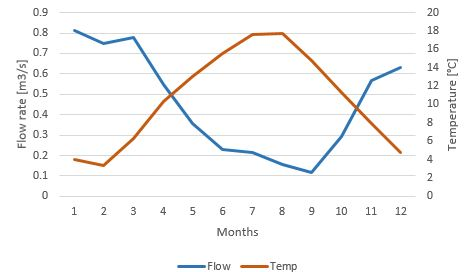
\includegraphics[width=1\textwidth]{river.JPG}
\caption{Temperature and flow of the Morges river}
\label{fig:river}
\end{figure}

According to this graph, it could be thought of using this river as a heat source for the heat pumps. However, what is not displayed is the minimum values. In fact, during droughts, the flow rate would not be sufficient to cover the heating/cooling demand. In fact, the lowest value has been reached in August 2004 with $0.017 m^3/s$, and even in December 2005 the lowest daily flow was of $0.057 m^3/s$. \\
For this reason, the stream has been excluded from further analysis and has not been considered as a viable solution.

\subsubsection{Lake}

\subsubsection{Geothermal wells}
Geothermal
Ground temperature shown in Figure \ref{fig:GTW_temp}.
Extracting power

100 CHF/m
http://bawos.ch/erdsondenbohrungen-kosten-und-planung-zur-gewinnung-von-umgebungswaerme/ 
https://www.energieheld.ch/heizung/waermepumpe/sole-wasser-erdwaerme 
Average 30 W/m
Heating 100/30 = 3600 CHF/kW
Th conductivity = 2.5 W/mk 
papers 
\begin{itemize}
\item between 2-5 \cite{jiaReviewEffectiveThermal2019}
\item other papers, check models for DX
\end{itemize}
$dT_{min}^{ref/ground} = 11 \si{\celsius}$

\begin{figure}[h!]
\centering
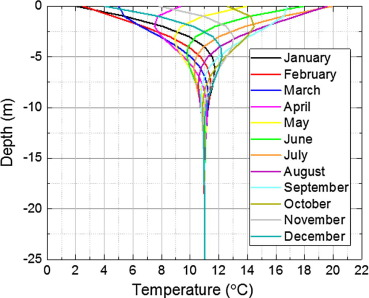
\includegraphics[width=1\textwidth]{GTW_temp.jpg}
\caption{Graphical representation of ground temperature, for different months of the year. Source: \cite{hanSensitivityAnalysisVertical2016}}
\label{fig:GTW_temp}
\end{figure}

$dT_water$ drop in ground loop is 3-5 \si{\celsius} for heating and 5-8 rise for cooling \cite{lundDESIGNCLOSEDLOOPGEOTHERMAL}
SIA makes an example with 3 \cite{siaSIA384Sondes2010}
$dT_{min} $ \cite{lundDESIGNCLOSEDLOOPGEOTHERMAL} with 15-16deg
\subsection{External heat sources}
The main advantage of a 5th generation district heating network is the ability to recover heat, and exchange it among the diversity of user. In the case of the Eglantine project, inside the district there are only very small heat sources and it is thus necessary to identify potential heat sources, located in the surroundings. 
Two potential heat sources have been identified:
\begin{itemize}
    \item The ice rink
    \item The shopping mall
\end{itemize}

\subsubsection{Ice rink}

\begin{figure}[h!]
\centering
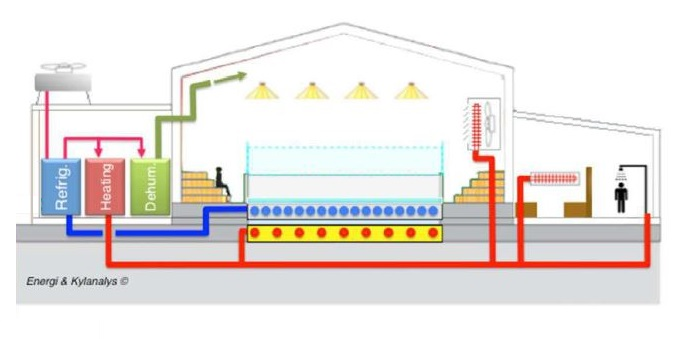
\includegraphics[width=1\textwidth]{IR_schema.JPG}
\caption{Energy system of a typical ice rink \cite{gronqvistComparativeLifecycleCost}}
\label{fig:IR_schema}
\end{figure}

An ice rink is a place where people can ice skate and play winter sports. The ice surface is normally inside an arena, which ensures comfortable temperatures for the people on the ice, as well as for the public, throughout the season. This also allows to extend the season, avoiding ice melt, when temperatures are warmer outside. A refrigeration system is responsible for the cooling of the ice surface. However, the ice rink often also includes changing rooms with showers, and a cafeteria or a restaurant. Thus, there is also need for heating. Furthermore, the ice surface has to be constantly illuminated, which requires a powerful lightning system. The global system is shown in Figure \ref{fig:IR_schema}.\\

The refrigeration of the ice surface leads to a high amount of waste heat, which is normally, or at least in older systems, exchanged with the environment. Connecting it to a 5th generation district heating network, would enable to recover this heat and use it to cover heat demand of other users.\\

The energy consumption of the ice rink has been estimated through a comparison of existing ice rinks in Sweden, which seems to be the only country for which the data is available and has been studied thoroughly.


Ice rinks normally cooled with indirect system, which is shown in the right part of Figure \ref{fig:IR_refSystem}

\begin{figure}[h!]
\centering
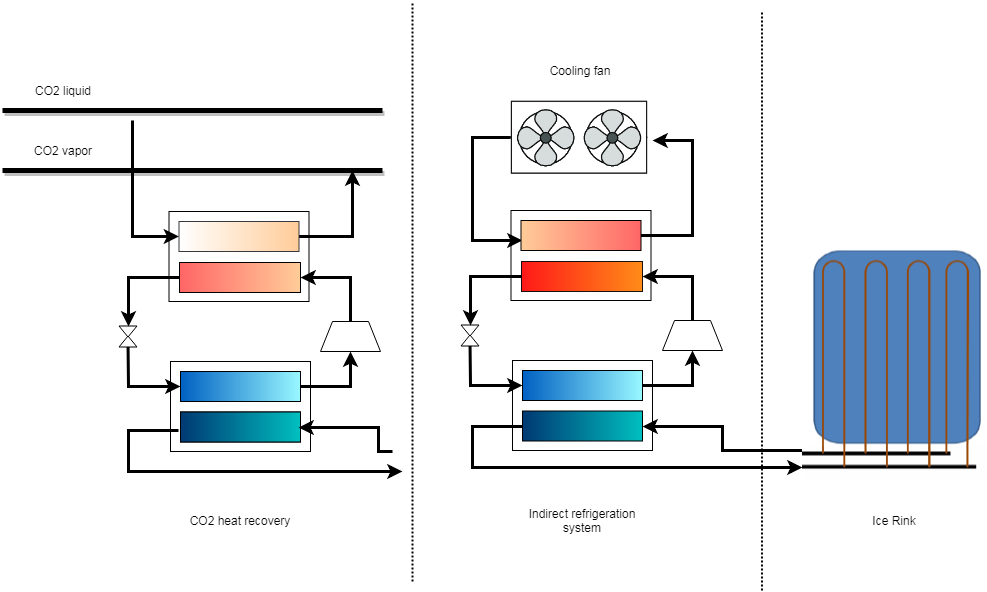
\includegraphics[width=1\textwidth]{IceRink_refrigeration.png}
\caption{Refrigeration systems for ice rinks}
\label{fig:IR_refSystem}
\end{figure}

this allows to use any refrigerant, since it won't come close to human activity. The most common refrigerant, at least in installed systems, is NH3, ammonia. Natural refrigerants, as for example CO2, are also becoming more common in new installations. 
The connection to the CO2 network is shown in the left part of Figure \ref{fig:IR_refSystem}.

A study, conducted on more than one hundred ice rinks in Sweden, shows that the refrigeration system has the largest share in total energy consumption, 43\% (in average) as indicated in Figure 8. (Rogstam (a), 2010) Heating with 26\% share is the second biggest energy consumer.
\cite{karampourMEASUREMENTMODELLINGICE}

\begin{figure}[h!]
\centering
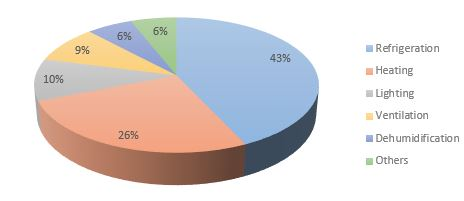
\includegraphics[width=0.7\textwidth]{IR_energyDemand.JPG}
\caption{Energy demand of a typical ice rink \cite{karampourMEASUREMENTMODELLINGICE}}
\label{fig:IR_energyDemand}
\end{figure}

The energy demand depends on the temperature of the ice. A typical temperature profile is shown in Table \ref{tab:IR_profile} \cite{karampourMEASUREMENTMODELLINGICE}.
\begin{table}[h]
\centering
\label{tab:IR_profile}
\caption{Ice rink refrigeration profile}\vspace{2mm} 
\begin{tabular}{lll}
\toprule
\textbf{Period} & \textbf{Rink function} & \textbf{\begin{tabular}[c]{@{}l@{}}$T_{ice}$\\ {[}\si{\celsius}{]}\end{tabular}} \\
\midrule 
0.00-6:00   & Night setback   & -1     \\
6:00-8:00   & Ice maintenance & -1     \\
8:00-16:00  & Low load        & -3     \\
16:00-18:00 & Figure skating  & -4     \\
18:00-24:00 & Hockey          & -6    \\
\bottomrule
\end{tabular}
\end{table}

From sources we have estimated a refrigeration profile shown in Figure ...
With the following assumptions:
\begin{itemize}
    \item Constant load profile throughout the ice season
    \item Ice season: 1st of August - 1st of April
    \item $COP_{ref} = 4$ \cite{karampourMEASUREMENTMODELLINGICE}
    \item Total waste heat = $ 1000 MWh/year$ \cite{kolasniewskiEvaluationModellingIce}
    \item $dT_{min}(refrigerant-ice) = 1 \si{\celsius}$
    \item $dT_{min}(refrigerant-refrigerant) = 3 \si{\celsius}$
\end{itemize}

\missingfigure{add figure with load profile... superpose temperature on second axis?}
% \begin{figure}[h!]
% \centering
% 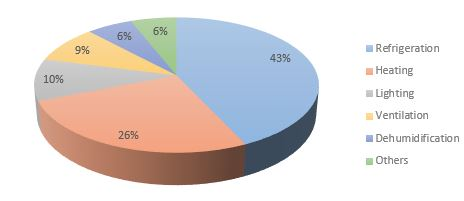
\includegraphics[width=0.7\textwidth]{IR_energyDemand.JPG}
% \caption{Energy demand of a typical ice rink \cite{karampourMEASUREMENTMODELLINGICE}}
% \label{fig:IR_energyDemand}
% \end{figure}

An new and efficient cooling system, together with an intelligent (weather, use, conditions...) management system, can drastically reduce energy consumption. This should be considered in the inclusion of the ice rink as heat source, since the renovation of the existing ice rink, or the construction of a new ice rink, would considerably reduce the amount of available waste heat.

\subsubsection{Shopping mall}

\subsection{Analysis/Extrapolation scenario}
A scenario to study parameters independently from Eglantine.
Parameters to study/extrapolate for quick application on other districts:
\begin{itemize}
    \item influence on IC,OC,TC
    \item influence on network temperature $T_net$  
\end{itemize}
Varying \% of cooling load, wrt heating load, using varying composition of cities, with categories (commercial/residential/...)


\section{Results}

\subsection{Scenario comparison}
\missingfigure[]{IC, OC, el consumption...}
Comparison with existing anergy networks, shown in Table \ref{tab:anergynets_IC}.
\begin{table}[h!]
\centering
\caption{Cost comparison with existing anergy systems}\vspace{2mm}
\label{tab:anergynets_IC} 
\begin{tabular}{llrrr}  \toprule
	&          & Eglantine & \begin{tabular}[c]{@{}l@{}}Anergienetz \\ ETH Hönggerberg\end{tabular} & \begin{tabular}[c]{@{}l@{}}Anergienetz \\ Friesenberg\end{tabular} \\ \midrule
	$IC_{NET}$             & [\%]     & 33.6 \%    & 15.7 \%                                                                 & 25.9 \%                                                             \\
	$IC_{GTW}$             & [\%]     & 44.6 \%    & 32.7 \%                                                                 & 23.5 \%                                                             \\
	$IC_{Heating/Cooling}$ & [\%]     & 21.8 \%    & 49.2 \%                                                                 & 50.6 \%                                                             \\
	Heating power          & [kW]     & 592       & 8'000                                                                  & 3'930                                                              \\
	Heating demand         & [MWh/yr] & 2'390     & 28'450                                                                 & 35'000                                                             \\
	Cooling power          & [kW]     & 84        & 6'000                                                                  & 3'500                                                              \\
	Cooling demand         & [MWh/yr] & 33        & 26'200                                                                 & 80'000                                                             \\ \bottomrule
%	Tot. Cost (excl. PV)   & [mioCHF] & 1.65      & 37                                                                     & 43                                                                
\end{tabular}
\end{table}

\subsection{CO2 network temperature control}
An optimum for the temperature of the CO2 network has been defined \todo{missing ref}.
The question arises if this temperature might vary in function of the operating condition of the network, i.e. the balance of heating and cooling load, the heat source temperature...\\
A model has been implemented to study this, by leaving the optimizer choose the optimal operating temperature of the network for every given timestep.\\
The results show that...
\missingfigure{graph of $Temp_net(time)$}
Then a simple representative scenario has been modeled, with a typical building, and a typical refrigeration, and varying \% of cooling load, wrt heating load.
\missingfigure{graph of $Temp_net$(\% of cooling/heating)}

\subsection{Sensitivity analysis}
Perform sensitivity analysis on:
\begin{itemize}
    \item PV area
    \item distance of lake
    \item size of Heat source (IceRink)
    \item distance of IceRink
    \item other ideas?
\end{itemize}

\section{Discussion}

\section{Outlook}
This and this has been analyzed and results have shown.\\
However, it would be very interesting to make detailed analysis of...\\
This model should be improved...\\
This new thing could be integrated...\\

\section{Conclusion}


%%%%%%%%% References %%%%%%%%%
\clearpage
\bibliographystyle{unsrt} %other styles: https://www.sharelatex.com/learn/Bibtex_bibliography_styles
\bibliography{bibliography.bib}

%%%%%%%%% Appendices %%%%%%%%%
\clearpage
\section{Anergy nets Switzerland}
\label{as:anergy_suisse}
\begin{landscape}
\begin{table}[h]
\centering
\caption{District energy systems in Switzerland ~\cite{energieschweizFallbeispieleThermischeNetze2018}; \textit{n/a}: not available}\vspace{2mm} 
\label{tab:anergieCH1} 
\begin{tabular}{llllllll}
\toprule
                                                                               & \textbf{\begin{tabular}[c]{@{}l@{}}Anergienetz \\ ETH \\ Hönggerberg\end{tabular}} & \textbf{\begin{tabular}[c]{@{}l@{}}Jardins de \\ la Pâla\end{tabular}}      & \textbf{\begin{tabular}[c]{@{}l@{}}Suurstoffi-\\ Areal\end{tabular}}                                  & \textbf{\begin{tabular}[c]{@{}l@{}}Anergienetz \\ Friesenberg (FGZ)\end{tabular}} & \textbf{\begin{tabular}[c]{@{}l@{}}CAD La-\\ Tour-De-Peilz\end{tabular}} & \textbf{\begin{tabular}[c]{@{}l@{}}Anergienetz-\\ Visp\end{tabular}}  & \textbf{\begin{tabular}[c]{@{}l@{}}Genève-Lac-\\ Nations (GLN)\end{tabular}}  \\
                                                                               \midrule
\textbf{Location}                                                              & Zürich                                                                             & Bulle                                                                       & Rotkreuz                                                                                              & Zürich                                                                            & La-Tour-de-Peilz                                                         & Visp                                                                  & Genève                                                                        \\
\textbf{Year of construction}                                                  & 2012 - 2026                                                                        & 2012 - 2020                                                                 & 2010 - 2020                                                                                           & 2011-2050                                                                         & 2013 - 2015                                                              & 2007 - heute                                                          & 2008 - 2016                                                                   \\
\textbf{Type}                                                                  & $\leq$ 20 \si{\celsius}                                                                            & $\leq$ 20 \si{\celsius}                                                                     & $\leq$ 20 \si{\celsius}                                                                                               & $\leq$ 20 \si{\celsius}                                                                           & $\leq$ 20\si{\celsius}                                                                   & $\leq$ 20 \si{\celsius}                                                               & $\leq$ 20 \si{\celsius}                                                                       \\
\textbf{Energy Ref. Area $[m2]$}                                                              & 475'000                                                                            & 65‘000                                                                      & 172'421                                                                                               & 185'000                                                                           & 24 Buildings                                                             & 160'000                                                               & 840'000                                                                       \\
\textbf{Use}                                                                   & \begin{tabular}[c]{@{}l@{}}School\\ Residential\end{tabular}                       & \begin{tabular}[c]{@{}l@{}}Residential\\ Commercial\\ Industry\end{tabular} & \begin{tabular}[c]{@{}l@{}}Residential\\ Administration\\ Commercial\\ Catering\\ School\end{tabular} & \begin{tabular}[c]{@{}l@{}}Residential\\ Computation\end{tabular}                 & \begin{tabular}[c]{@{}l@{}}Residential\\ Administration\end{tabular}     & \begin{tabular}[c]{@{}l@{}}Residential\\ Industry\end{tabular}        & \begin{tabular}[c]{@{}l@{}}Residential\\ Administration\\ School\end{tabular} \\
\textbf{Status}                                                                & Partly built                                                                       & Partly built                                                                & Partly built                                                                                          & Partly built                                                                      & Built                                                                    & Built                                                                 & Built                                                                         \\
\midrule
\textbf{}                                                                      & \multicolumn{7}{c}{Data Energy Consumption}                                                                                                                                                                                                                                                                                                                                                                                                                                                                                                                                                     \\
\midrule
\textbf{\begin{tabular}[c]{@{}l@{}}Inst. Heating\\ capacity $[kW]$\end{tabular}} & 8'000                                                                              & 2'000                                                                       & 6'732                                                                                                 & 3'930                                                                             & 10'000                                                                   & 3'467                                                                 & 4'300                                                                         \\
\textbf{\begin{tabular}[c]{@{}l@{}}Heating demand \\ $[MWh/a]$\end{tabular}}   & 28'450                                                                             & 3'100                                                                       & 10'619                                                                                                & 35'000                                                                            & 812                                                                      & 8'737                                                                 & 5’000                                                                         \\
\textbf{\begin{tabular}[c]{@{}l@{}}Inst. Cooling\\ capacity $[kW]$\end{tabular}} & 6'000                                                                              & 1'000                                                                       & 2'327                                                                                                 & 3'500                                                                             & None                                                                     & 2'600                                                                 & 16'200                                                                        \\
\textbf{\begin{tabular}[c]{@{}l@{}}Cooling demand \\ $[MWh/a]$\end{tabular}}   & 26'200                                                                             & 650                                                                         & 2'364                                                                                                 & 80'000                                                                            & None                                                                     & 3'380                                                                 & 20'000                                                                        \\
\textbf{Heat source}                                                           & \begin{tabular}[c]{@{}l@{}}Laboratories\\ waste heat \\ +HP\end{tabular}           & Groundwater+HP                                                              & \begin{tabular}[c]{@{}l@{}}Waste heat \\ buildings \\ + PVT (solar th.) \\ +HP\end{tabular}           & \begin{tabular}[c]{@{}l@{}}Waste heat\\ data center+HP\end{tabular}               & Lake water +HP                                                           & \begin{tabular}[c]{@{}l@{}}Inudstrial waste \\ heat + HP\end{tabular} & Lake water +HP                                                                \\
\textbf{Heat storage}                                                          & \begin{tabular}[c]{@{}l@{}}Geothermal well \\ field\\ (431 at 200m)\end{tabular}   & Groundwater 12\si{\celsius}                                                            & \begin{tabular}[c]{@{}l@{}}Geothermal well\\ field \\ (215 at 150 m,\\ 180 at 280m)\end{tabular}      & \begin{tabular}[c]{@{}l@{}}Geothermal well\\ field\\ (332 at 250m)\end{tabular}   & None                                                                     & None                                                                  & None                                                                          \\
\midrule
\textbf{}                                                                      & \multicolumn{7}{c}{Network data}                                                                                                                                                                                                                                                                                                                                                                                                                                                                                                                                                                \\
\midrule
\textbf{Network length $[km]$}                                                   & 1.5                                                                                & 0.85                                                                        & 2.5                                                                                                   & 1.5                                                                               & 4.1                                                                      & 4.2                                                                   & 6                                                                             \\
\textbf{Heating pipeT}                                                         & 24 \si{\celsius} - 8 \si{\celsius}                                                                       & 12 \si{\celsius} - 9 \si{\celsius}                                                                & 25 \si{\celsius} - 8 \si{\celsius}                                                                                          & 28 \si{\celsius} - 8 \si{\celsius}                                                                      & 20 \si{\celsius} - 6 \si{\celsius}                                                             & 18 \si{\celsius} - 8 \si{\celsius}                                                          & 17 \si{\celsius} - 5 \si{\celsius}                                                                  \\
\textbf{Cooling pipeT}                                                         & 4 \si{\celsius} - 20 \si{\celsius}                                                                       & 4 \si{\celsius} - 17 \si{\celsius}                                                                & 4 \si{\celsius} - 17 \si{\celsius}                                                                                          & 4 \si{\celsius} -24 \si{\celsius}                                                                       & 2 \si{\celsius} - 16 \si{\celsius}                                                             & 4 \si{\celsius} - 16 \si{\celsius}                                                          & 5 \si{\celsius} - 12 \si{\celsius}                                                                  \\
\textbf{Pipe diameter $[mm]$}                                                    & DN 560                                                                             & 75 - 250                                                                    & 60 - 400                                                                                              & 400 - 500                                                                         & 400 -700                                                                 & DN 400                                                                & 100 -700                                                                      \\
\textbf{Number of pipes}                                                       & 3                                                                                  & 2                                                                           & 2                                                                                                     & 2                                                                                 & 2                                                                        & 2                                                                     & 2       \\
\bottomrule
\end{tabular}
\end{table}

\end{landscape}
\begin{landscape}
\begin{table}[h]
\centering
\caption{District energy systems in Switzerland}\vspace{2mm}
\label{tab:anergieCH2} 
\begin{tabular}{llllllll}
\toprule

                                                                                      & \textbf{\begin{tabular}[c]{@{}l@{}}Anergienetz \\ ETH \\ Hönggerberg\end{tabular}} & \textbf{\begin{tabular}[c]{@{}l@{}}Jardins de \\ la Pâla\end{tabular}}             & \textbf{\begin{tabular}[c]{@{}l@{}}Suurstoffi-\\ Areal\end{tabular}} & \textbf{\begin{tabular}[c]{@{}l@{}}Anergienetz \\ Friesenberg (FGZ)\end{tabular}} & \textbf{\begin{tabular}[c]{@{}l@{}}CAD La-\\ Tour-De-Peilz\end{tabular}}      & \textbf{\begin{tabular}[c]{@{}l@{}}Anergienetz-\\ Visp\end{tabular}} & \textbf{\begin{tabular}[c]{@{}l@{}}Genève-Lac-\\ Nations (GLN)\end{tabular}} \\
                                                                                      \midrule
\textbf{}                                                                             & \multicolumn{7}{c}{Financial data}                                                                                                                                                                                                                                                                                                                                                                                                                                                                                                                                       \\
\midrule
\textbf{\begin{tabular}[c]{@{}l@{}}Tot. investments\\ '[Mio.CHF]'\end{tabular}}       & 37                                                                                 & 6                                                                                  & n/a                                                                  & 42.5                                                                              & 32                                                                            & 1.26                                                                 & 33                                                                           \\
\textbf{Interest rate[\%]}                                                            & 3.9 - 6.7                                                                          &                                                                                    & n/a                                                                  & n/a                                                                               & 6.4                                                                           & 5.8 - 8                                                              & n/a                                                                          \\
\textbf{Lifespan [a]}                                                                 &                                                                                    &                                                                                    &                                                                      &                                                                                   &                                                                               &                                                                      &                                                                              \\
\textbf{Pipes}                                                                        & 50                                                                                 & 30                                                                                 & 40                                                                   & 50                                                                                & 50                                                                            & 40                                                                   & n/a                                                                          \\
\textbf{Storage}                                                                      & 50                                                                                 & None                                                                               & 80                                                                   & 50                                                                                & None                                                                          & None                                                                 & n/a                                                                          \\
\textbf{Heating unit}                                                                 & 20                                                                                 & 15                                                                                 & 20                                                                   & 20                                                                                & 25                                                                            & 20                                                                   & n/a                                                                          \\
\textbf{Cooling unit}                                                                 & 20                                                                                 & 15                                                                                 & 20                                                                   & 20                                                                                & 25                                                                            & 20                                                                   & n/a                                                                          \\
\textbf{\begin{tabular}[c]{@{}l@{}}Cost of energy \\ '[Rp./kWh]'\end{tabular}}        & \begin{tabular}[c]{@{}l@{}}7.7 \\ (Heating +cooling)\end{tabular}                  & \begin{tabular}[c]{@{}l@{}}5.85 – 8\\ (at the moment \\ only heating)\end{tabular} & n/a                                                                  & \begin{tabular}[c]{@{}l@{}}18\\ (Heating)\end{tabular}                            & \begin{tabular}[c]{@{}l@{}}19.8\\ (at the moment\\ only heating)\end{tabular} & \begin{tabular}[c]{@{}l@{}}22.9\\ (Heating +\\ cooling)\end{tabular} & n/a                                                                          \\
\textbf{Tot. COP of heating}                                                          & 7.2                                                                                & 4.4                                                                                & n/a                                                                  & 5.2                                                                               & n/a                                                                           & n/a                                                                  & n/a                                                                          \\
\textbf{\begin{tabular}[c]{@{}l@{}}Tot. COP of heating\\ (incl. Pumps…)\end{tabular}} & 5.8                                                                                & 2.7                                                                                & 2.7                                                                  & 4.1                                                                               & 3.5-4                                                                         & 4                                                                    & 6.5                                                                          \\
\textbf{Tot. EER of cooling}                                                          & 30.1                                                                               & n/a                                                                                & n/a                                                                  & n/a                                                                               & n/a                                                                           & n/a                                                                  & n/a                                                                          \\
\textbf{\begin{tabular}[c]{@{}l@{}}Tot. EER of cooling\\ (incl. Pumps…)\end{tabular}} & 6.9                                                                                & 12.1                                                                               & n/a                                                                  & n/a                                                                               & n/a                                                                           & n/a                                                                  & n/a \\
\bottomrule
\end{tabular}
\end{table}

\end{landscape}


%%%%%%%%%%%%%%%%%%%%%%%%%%%% END %%%%%%%%%%%%%%%%%%%%%%%%%%%%%%%%%%%
\end{document}
